\documentclass[journal, 10pt, twoside]{IEEEtran}

% ── Packages ──────────────────────────────────────────────────────────────────
\usepackage[T1]{fontenc}
\usepackage[utf8]{inputenc}
\usepackage{amsmath, amssymb}
\usepackage{graphicx}
\usepackage{booktabs}
\usepackage{multirow}
\usepackage{array}
\usepackage{xcolor}
\usepackage{hyperref}
\usepackage{cite}
\usepackage{balance}
\usepackage{microtype}
\usepackage{float}
\usepackage[caption=false, font=footnotesize]{subfig}

\graphicspath{{./}}   % figures live in the same reports/ folder

% ── Hyperref ──────────────────────────────────────────────────────────────────
\hypersetup{
  colorlinks = true,
  linkcolor  = blue!60!black,
  citecolor  = green!50!black,
  urlcolor   = blue!60!black,
}

% ══════════════════════════════════════════════════════════════════════════════
\begin{document}

% ── Title & Authors ───────────────────────────────────────────────────────────
\title{Automated Brugada Syndrome Detection from 12-Lead ECG\\
       Using Classical Machine Learning and Deep Neural Networks}

\author{%
  \IEEEauthorblockN{Aisya Ulul Asmi\IEEEauthorrefmark{1} and
                    Fiqki Haidar Amrullah\IEEEauthorrefmark{1}}
  \IEEEauthorblockA{\IEEEauthorrefmark{1}%
    Department of Intelligent Data Science and Computation,\\
    \textit{Email: \{aisya.asmi, fiqki.amrullah\}@student.ac.id}}
}

\maketitle

% ── Abstract ──────────────────────────────────────────────────────────────────
\begin{abstract}
Brugada syndrome (BrS) is a rare but life-threatening inherited channelopathy
characterised by a coved ST-elevation pattern in the right precordial leads
(V1--V3) of the standard 12-lead electrocardiogram (ECG).
Missed diagnosis can lead to sudden cardiac death.
This paper presents an end-to-end automated detection pipeline evaluated on
the PhysioNet Brugada-HUCA dataset (363 patients: 69 BrS, 294 Normal).
Seven classifiers are compared across two paradigms:
classical machine learning (Logistic Regression, Random Forest) operating
on 207 handcrafted features, and five end-to-end deep learning architectures
(1D ResNet, 1D CNN, 1D RNN, BiLSTM, LSTM).
The 1D ResNet achieves the best \textit{overall} performance with
\textbf{AUROC = 0.9574}, \textbf{F1 = 0.8462},
sensitivity = 91.7\%, and specificity = 93.0\% on the held-out test set.
Notably, the 1D CNN achieves the highest AUROC (0.9767) and AUPRC (0.9493)
with a substantially smaller parameter count, making it a strong
lightweight alternative when computational resources are constrained.
Model decisions are explained via SHAP (Random Forest) and GradCAM
(1D ResNet), both confirming that the models focus on the clinically
expected V1/V2/V3 leads and the ST-segment region.
A reduced-lead ablation study further demonstrates that full 12-lead
recordings provide substantially higher specificity and F1 compared
to V1--V2 (+24.6 pp F1) or V1--V3 (+28.6 pp F1) subsets.
\end{abstract}

\begin{IEEEkeywords}
Brugada syndrome, ECG classification, 1D ResNet, 1D CNN, LSTM,
SHAP, GradCAM, reduced-lead ablation, imbalanced learning.
\end{IEEEkeywords}

% ══════════════════════════════════════════════════════════════════════════════
\section{Introduction}
\label{sec:intro}

Brugada syndrome (BrS) is an autosomal-dominant cardiac ion-channel disorder
associated with a markedly elevated risk of ventricular fibrillation and
sudden cardiac death in structurally normal hearts \cite{brugada1992right}.
The estimated prevalence ranges from 1:2000 to 1:5000 in the general
population, with higher incidence in South-East Asia \cite{antzelevitch2005brugada}.
The diagnostic hallmark is a Type-1 coved ST-elevation of $\geq 2$\,mm
in at least one right precordial lead (V1 or V2), either spontaneously
or after sodium-channel blocker challenge \cite{priori2013hrs}.

Despite the distinctive ECG pattern, BrS is frequently missed in routine
clinical practice due to its dynamic and intermittent expression, the
subtle morphology differences between Type-1 (coved) and Type-2 (saddle-back)
patterns, and the high daily volume of ECGs reviewed by cardiologists.
Computer-aided ECG interpretation systems can assist by automatically
flagging recordings with suspicious patterns for expert review, thereby
reducing missed diagnoses and accelerating the diagnostic pathway.

Recent advances in deep learning have demonstrated strong performance on
ECG classification tasks \cite{hannun2019cardiologist, ribeiro2020automatic},
yet studies focused specifically on BrS detection remain scarce and often
limited to small datasets or single-lead analysis.
This work addresses that gap with the following contributions:

\begin{enumerate}
  \item A reproducible end-to-end pipeline (preprocessing $\to$ feature
        extraction $\to$ training $\to$ threshold optimisation $\to$
        interpretability) on a publicly available BrS dataset.
  \item A broad comparison of seven classifiers spanning classical ML
        and five deep learning architectures (1D ResNet, 1D CNN, RNN,
        BiLSTM, LSTM) for BrS detection.
  \item A computational efficiency analysis identifying the 1D CNN as
        a strong lightweight alternative to the 1D ResNet when
        resources are constrained.
  \item Clinically grounded interpretability using SHAP and GradCAM,
        validating that learned features align with medical knowledge.
  \item A reduced-lead ablation study quantifying the trade-off between
        lead count and diagnostic performance.
\end{enumerate}

% ══════════════════════════════════════════════════════════════════════════════
\section{Dataset}
\label{sec:dataset}

\subsection{PhysioNet Brugada-HUCA}

The Brugada-HUCA dataset \cite{dataset} (v1.0.0) is a single-centre
collection from the Hospital Universitari Central d'Astúries (HUCA), Spain,
available on PhysioNet \cite{physionet}.
It contains 363 resting 12-lead ECG recordings sampled at 100\,Hz,
each 12 seconds long (1200 samples per lead).
Labels are binary: 1 for Type-1 or Type-2 Brugada syndrome,
0 for Normal.

\begin{table}[h]
  \centering
  \caption{Dataset statistics}
  \label{tab:dataset}
  \begin{tabular}{lcc}
    \toprule
    \textbf{Property} & \textbf{Value} \\
    \midrule
    Total patients       & 363 \\
    Brugada (positive)   & 69 (19.0\%) \\
    Normal (negative)    & 294 (81.0\%) \\
    Class imbalance      & 1\,:\,4.26 \\
    Sampling rate        & 100\,Hz \\
    Recording duration   & 12\,s (1200 samples) \\
    Number of leads      & 12 \\
    Diagnostic leads     & V1, V2, V3 \\
    \bottomrule
  \end{tabular}
\end{table}

\subsection{Class Imbalance}

The dataset is moderately imbalanced with a positive-to-negative ratio of
approximately 1:4.26.
This is handled at the algorithm level via a weighted loss function
($\text{pos\_weight} = n_\text{neg} / n_\text{pos} \approx 4.27$) for the
deep learning model, and via \texttt{class\_weight=balanced} for classical
classifiers.

\subsection{Data Splits}

All splits are performed at the patient level using stratified sampling
(seed = 42) to preserve the class ratio in each partition.
Table~\ref{tab:splits} reports the resulting subset sizes.

\begin{table}[h]
  \centering
  \caption{Train / Validation / Test splits}
  \label{tab:splits}
  \begin{tabular}{lcccr}
    \toprule
    \textbf{Split} & \textbf{N} & \textbf{BrS} & \textbf{Normal} & \textbf{BrS \%} \\
    \midrule
    Train      & 253 & 48 & 205 & 19.0\% \\
    Validation & 55  & 12 & 43  & 21.8\% \\
    Test       & 55  & 12 & 43  & 21.8\% \\
    \bottomrule
  \end{tabular}
\end{table}

% ══════════════════════════════════════════════════════════════════════════════
\section{Methods}
\label{sec:methods}

\subsection{Preprocessing Pipeline}

All raw signals are passed through the same three-stage pipeline
prior to model input:

\begin{enumerate}
  \item \textbf{Bandpass filter:} Fourth-order Butterworth filter
        (0.5--40\,Hz, zero-phase via \texttt{sosfiltfilt}).
        Removes baseline wander ($<$0.5\,Hz) and high-frequency
        muscle noise ($>$40\,Hz).
  \item \textbf{Notch filter:} 50\,Hz notch ($Q = 30$) to remove
        European powerline interference.
  \item \textbf{Z-score normalisation:} Per lead, per patient.
        Ensures zero mean and unit variance across each 12-second segment.
\end{enumerate}

\begin{figure}[H]
  \centering
  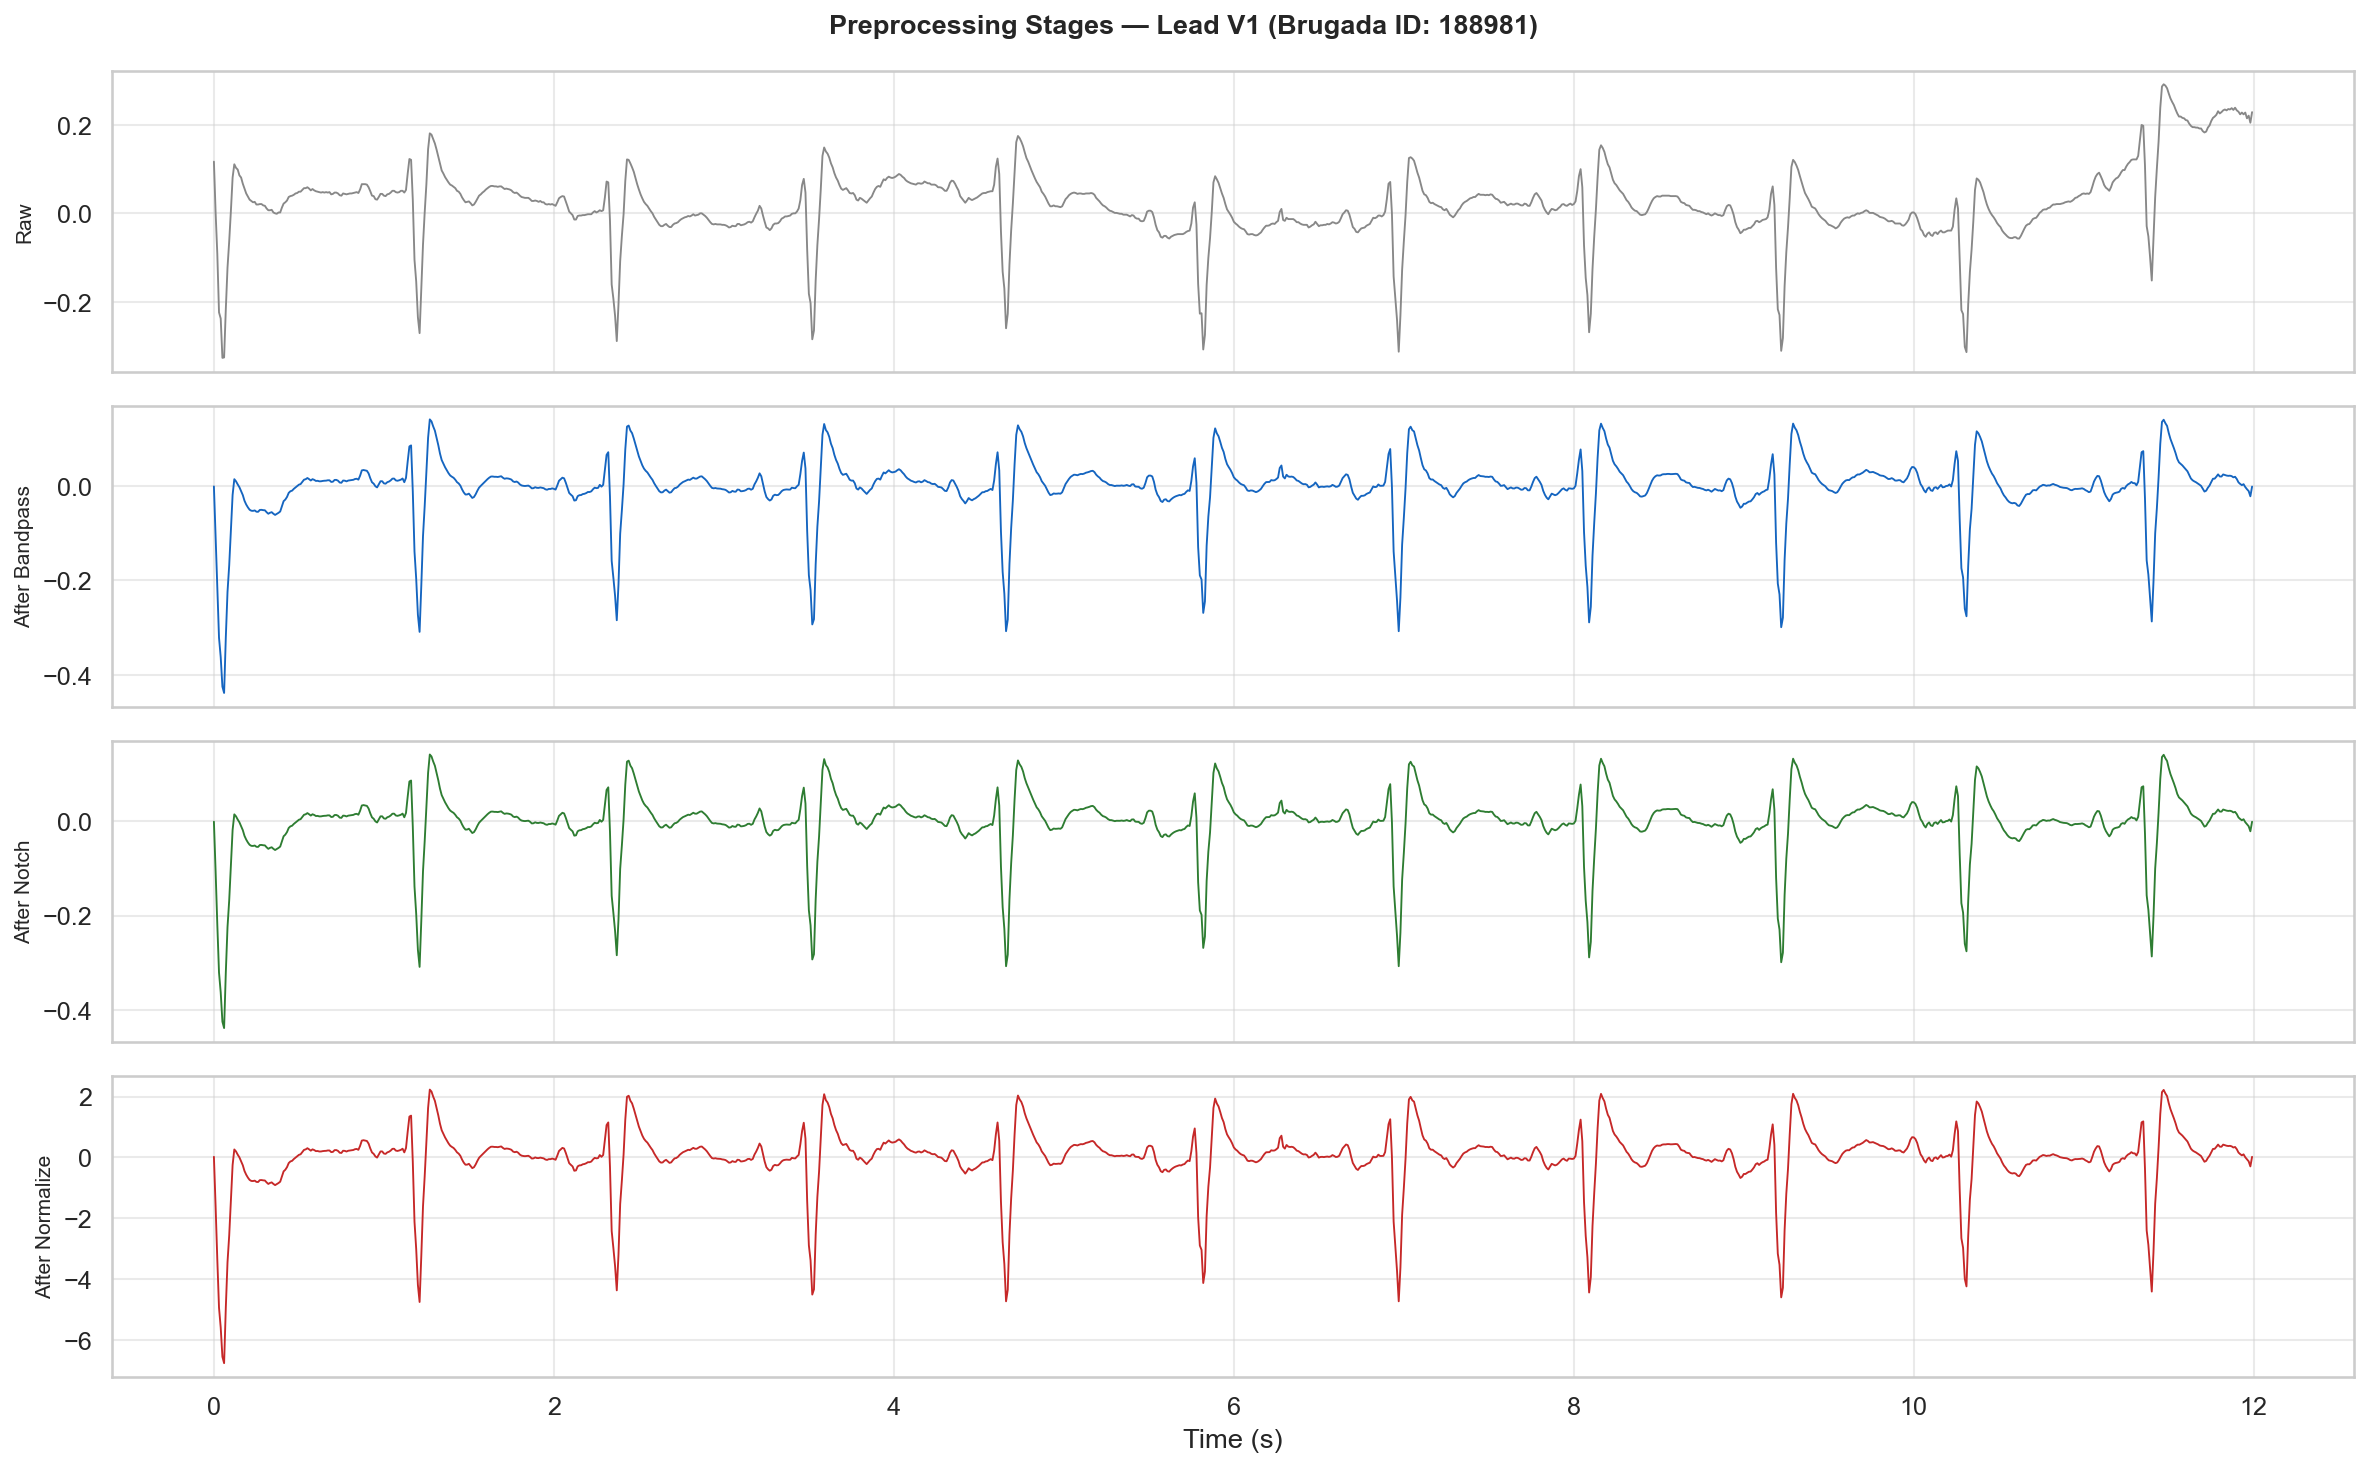
\includegraphics[width=\columnwidth]{preproc_filter_stages.png}
  \caption{Lead V1 signal through each preprocessing stage for one
           Brugada patient: raw $\to$ bandpass $\to$ notch $\to$ normalised.}
  \label{fig:filter_stages}
\end{figure}

\subsection{Data Augmentation}

To reduce overfitting given the small training set, three on-the-fly
augmentation operations are applied exclusively to the training set:
(i) additive Gaussian noise ($\sigma = 0.01$),
(ii) random time shift ($\pm 10$ samples), and
(iii) random amplitude scaling (uniform in $[0.9, 1.1]$).
Validation and test sets are always evaluated on clean signals.

\subsection{Feature Extraction for Classical Models}

For the Logistic Regression and Random Forest models, 207 handcrafted
features are extracted per patient across four groups:

\begin{itemize}
  \item \textbf{Time-domain} (108 features): mean, standard deviation,
        minimum, maximum, range, mean absolute value, RMS,
        skewness, and kurtosis computed per lead (9 $\times$ 12).
  \item \textbf{Frequency-domain} (72 features): total power and
        relative power in three bands (0.5--5\,Hz, 5--15\,Hz,
        15--40\,Hz) per lead (6 $\times$ 12).
  \item \textbf{Brugada morphology} (12 features): J-point amplitude,
        ST-segment elevation, ST slope, and coved ratio for V1, V2,
        and V3 (4 $\times$ 3).
  \item \textbf{Heart rate variability} (7 features): mean and standard
        deviation of HR and RR intervals, SDNN, RMSSD, and pNN50
        extracted from Lead~II.
\end{itemize}

All features are standardised using a \texttt{StandardScaler} fitted on
the training set only.

\subsection{Model Architectures}

\subsubsection{Logistic Regression (Baseline)}
Standard $L_2$-regularised logistic regression with $C = 0.1$
and \texttt{class\_weight=balanced}.
Operates on the 207-dimensional feature vector.

\subsubsection{Random Forest}
An ensemble of decision trees with hyperparameters selected by
5-fold stratified cross-validation (GridSearchCV) over:
$n_\text{estimators} \in \{200, 400\}$,
$\text{max\_depth} \in \{\text{None}, 15, 25\}$,
$\text{min\_samples\_leaf} \in \{1, 2\}$,
with \texttt{class\_weight=balanced}.

\subsubsection{1D Residual Network (ResNet1D)}

The primary deep learning model is a one-dimensional residual
convolutional network \cite{he2016deep} adapted for multi-lead ECG:

\begin{itemize}
  \item \textbf{Stem:} \texttt{Conv1d}($12 \to 64$, $k=15$, $s=2$)
        + BN + ReLU + MaxPool $\to$ $(B, 64, 300)$.
  \item \textbf{Layers 1--4:} Two residual blocks each, channel widths
        64/128/256/512 with progressive downsampling ($s=2$, layers 2--4).
        Each block: \texttt{Conv1d}$\to$BN$\to$ReLU$\to$Dropout(0.2)
        $\to$\texttt{Conv1d}$\to$BN + skip connection.
  \item \textbf{Head:} Global average pooling $\to$ Dropout(0.5) $\to$
        \texttt{Linear}$(512 \to 1)$.
\end{itemize}

Total trainable parameters: $\approx 1.4$ million.

\subsubsection{1D Convolutional Network (CNN1D)}

A plain (non-residual) 1D CNN with a shallower design than ResNet1D,
achieving competitive performance at a significantly lower parameter count:

\begin{itemize}
  \item \textbf{Block 1--4:} \texttt{Conv1d} with increasing channels
        (32, 64, 128, 256), $k=7$, BN, ReLU, MaxPool(2).
  \item \textbf{Head:} Global average pooling $\to$ Dropout(0.5) $\to$
        \texttt{Linear}$(256 \to 1)$.
\end{itemize}

The absence of residual connections reduces complexity while the
4-stage convolution stack retains sufficient receptive field for
the 12-second ECG signal.

\subsubsection{Recurrent Models (RNN1D, LSTM1D, BiLSTM1D)}

Three sequence models are evaluated to assess whether temporal
recurrence offers advantages over convolution for ECG classification.
All three receive the ECG as a sequence of 1200 time steps with 12
input features (one per lead):

\begin{itemize}
  \item \textbf{RNN1D:} Single-layer vanilla RNN (hidden size 128)
        $\to$ last hidden state $\to$ \texttt{Linear}$(128 \to 1)$.
  \item \textbf{LSTM1D:} Two-layer LSTM (hidden size 128, Dropout 0.3
        between layers) $\to$ last hidden state
        $\to$ \texttt{Linear}$(128 \to 1)$.
  \item \textbf{BiLSTM1D:} Two-layer bidirectional LSTM (hidden size 128
        per direction) $\to$ concatenated forward/backward final states
        $\to$ \texttt{Linear}$(256 \to 1)$.
\end{itemize}

All deep learning models share the same training protocol
described in Section~\ref{sec:training}.

\subsection{Training Protocol}
\label{sec:training}

All deep learning models are trained with:
\textbf{Loss:} \texttt{BCEWithLogitsLoss} with
$\text{pos\_weight} = 4.27$;
\textbf{Optimiser:} AdamW
($\text{lr} = 10^{-3}$, $\lambda = 10^{-4}$);
\textbf{Scheduler:} Cosine annealing
($T_\text{max} = 50$, $\eta_\text{min} = 10^{-5}$);
\textbf{Early stopping:} patience = 10 epochs on validation loss;
\textbf{Gradient clipping:} max-norm = 1.0;
\textbf{Batch size:} 32.

\begin{figure}[H]
  \centering
  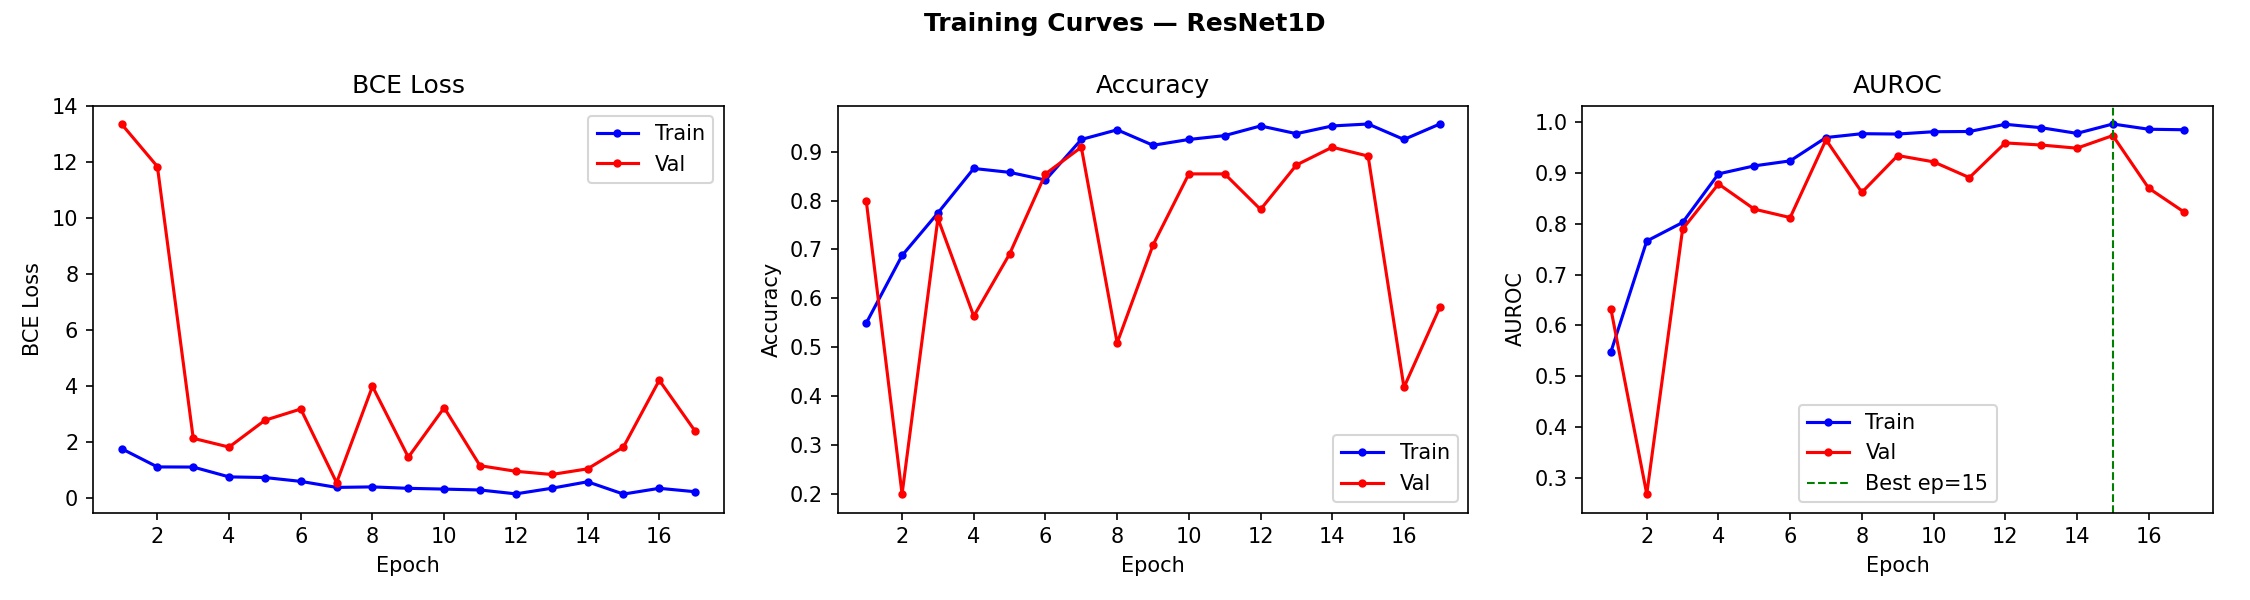
\includegraphics[width=\columnwidth]{training_curves.png}
  \caption{1D ResNet training history: loss, accuracy, and AUROC
           on train and validation sets over 50 epochs.}
  \label{fig:training_curves}
\end{figure}

\subsection{Decision Threshold Optimisation}

All models output a probability score $\hat{p} \in [0, 1]$.
The binary decision threshold $\tau$ is selected on the
\textit{validation set} by sweeping 100 candidate values in
$[0.01, 0.99]$ and choosing the $\tau$ that maximises $F_1$
subject to the clinical constraint:
\begin{equation}
  \tau^* = \arg\max_{\tau}\; F_1(\tau)
  \quad \text{s.t.} \quad \text{Sensitivity}(\tau) \geq 0.85.
  \label{eq:thresh}
\end{equation}
This constraint reflects the clinical priority of minimising
missed Brugada diagnoses (false negatives), which carry a higher
consequence than false positives.

% ══════════════════════════════════════════════════════════════════════════════
\section{Results}
\label{sec:results}

\subsection{Model Comparison on the Test Set}

Table~\ref{tab:results} reports all metrics computed on the held-out
test set (55 patients, 12 BrS, 43 Normal) at the threshold
$\tau^*$ optimised on the validation set.

\begin{table*}[t]
  \centering
  \caption{Test-set performance of all seven models (55 patients, 12 BrS, 43 Normal).
           Best value per column in \textbf{bold}. $\dagger$ lightweight alternative.}
  \label{tab:results}
  \renewcommand{\arraystretch}{1.25}
  \begin{tabular}{lccccccccc}
    \toprule
    \textbf{Model} & \textbf{Type}
      & \textbf{AUROC} & \textbf{AUPRC}
      & \textbf{Sens.} & \textbf{Spec.}
      & \textbf{Prec.} & \textbf{F1}
      & \textbf{Acc.}  & \textbf{$\tau^*$} \\
    \midrule
    Logistic Regression & Classical ML
      & 0.7345 & 0.5951
      & 83.3\% & 34.9\%
      & 26.3\% & 0.400
      & 45.5\% & 0.020 \\
    Random Forest & Classical ML
      & 0.9341 & 0.7848
      & \textbf{100.0\%} & 74.4\%
      & 52.2\% & 0.686
      & 80.0\% & 0.158 \\
    \midrule
    RNN1D & Deep Learning
      & 0.5465 & 0.3131
      & 50.0\% & 48.8\%
      & 21.4\% & 0.300
      & 49.1\% & 0.310 \\
    BiLSTM1D & Deep Learning
      & 0.8178 & 0.5465
      & 83.3\% & 60.5\%
      & 37.0\% & 0.513
      & 65.5\% & 0.200 \\
    LSTM1D & Deep Learning
      & 0.8934 & 0.7810
      & \textbf{100.0\%} & 37.2\%
      & 30.8\% & 0.471
      & 50.9\% & 0.250 \\
    CNN1D$^\dagger$ & Deep Learning
      & \textbf{0.9767} & \textbf{0.9493}
      & 91.7\% & 90.7\%
      & 73.3\% & 0.815
      & 90.9\% & 0.610 \\
    \textbf{ResNet1D} & Deep Learning
      & 0.9574 & 0.9351
      & 91.7\% & \textbf{93.0\%}
      & \textbf{78.6\%} & \textbf{0.846}
      & \textbf{92.7\%} & 0.770 \\
    \bottomrule
  \end{tabular}
\end{table*}

\textbf{ResNet1D} achieves the best overall balance:
highest F1 (0.846), specificity (93.0\%), precision (78.6\%),
and accuracy (92.7\%), with only 1 missed Brugada case (FN = 1)
and 3 false alarms (FP = 3).

\textbf{CNN1D} surpasses ResNet1D on both AUROC (0.9767 vs.\ 0.9574)
and AUPRC (0.9493 vs.\ 0.9351) while achieving identical sensitivity
(91.7\%) at a lower parameter count, making it a competitive lightweight
alternative (discussed further in Section~\ref{sec:cnn_vs_resnet}).

\textbf{Recurrent models} (RNN1D, LSTM1D, BiLSTM1D) perform poorly
relative to convolutional models.
RNN1D is near-random (AUROC = 0.5465), and LSTM1D achieves perfect
sensitivity only by setting a very low threshold (0.250), producing
27 false positives (specificity = 37.2\%).
BiLSTM1D performs better but remains well below the convolutional approaches.
This suggests that the local morphological patterns critical for BrS
detection are better captured by convolutional kernels than by
sequential state propagation.

\textbf{Classical models:} The Random Forest achieves perfect sensitivity
(zero missed BrS cases) via a low threshold (0.158), but generates
11 false positives.
The Logistic Regression is practically unusable as a standalone classifier
(specificity = 34.9\%, 28 false positives).

\begin{figure}[H]
  \centering
  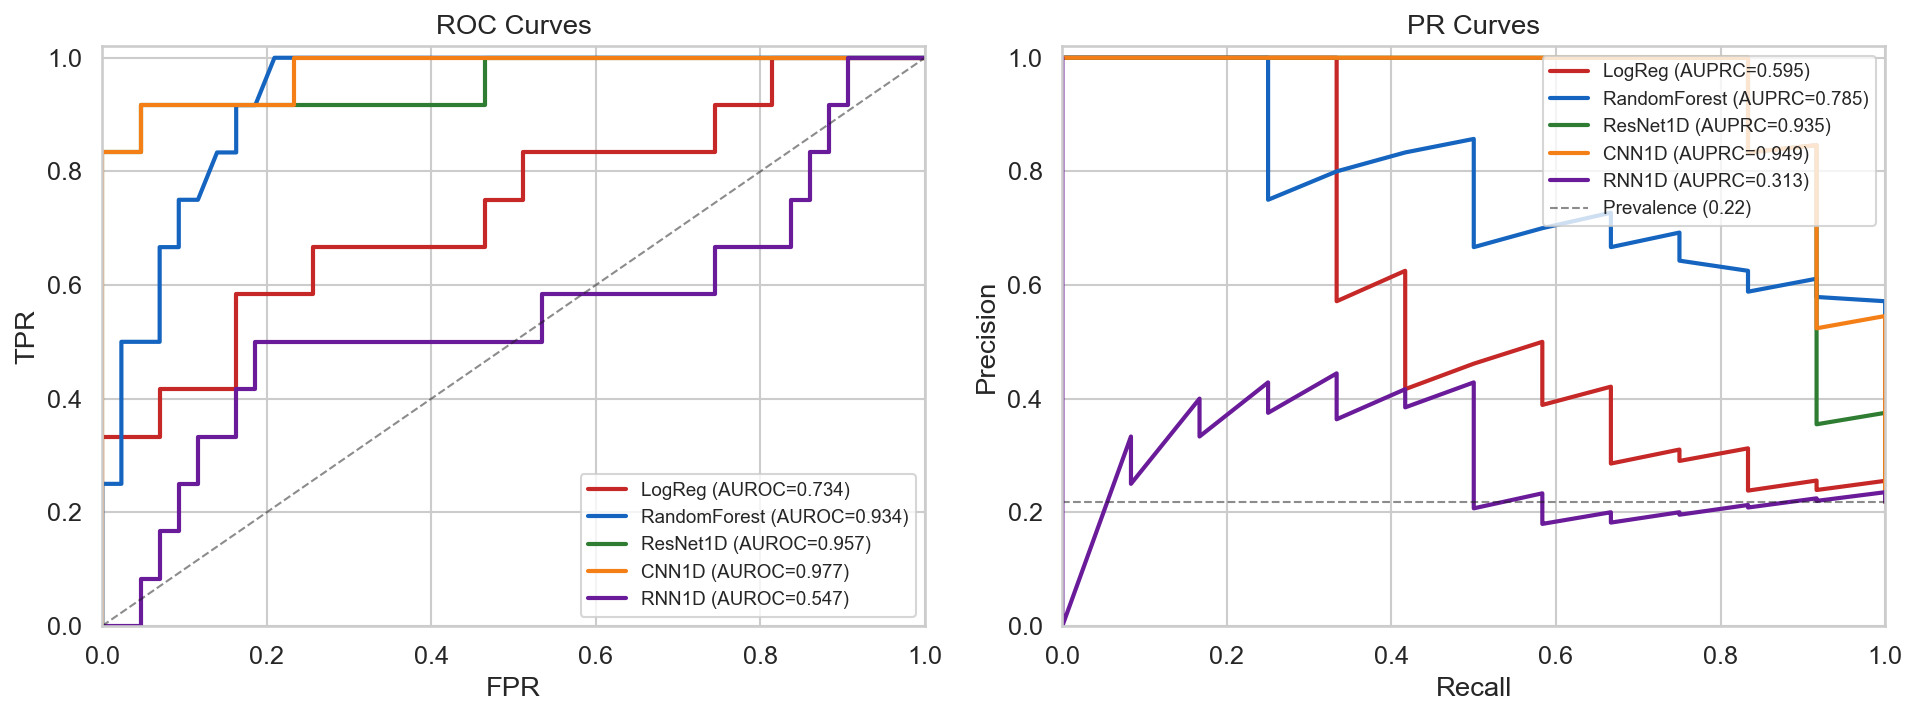
\includegraphics[width=\columnwidth]{eval_roc_pr_curves.png}
  \caption{ROC curves (left) and Precision-Recall curves (right) for
           all seven models on the test set. CNN1D (orange) achieves
           the highest area under both curves. The dashed line in the
           PR plot marks the dataset prevalence (0.22).}
  \label{fig:roc_pr}
\end{figure}

\begin{figure}[H]
  \centering
  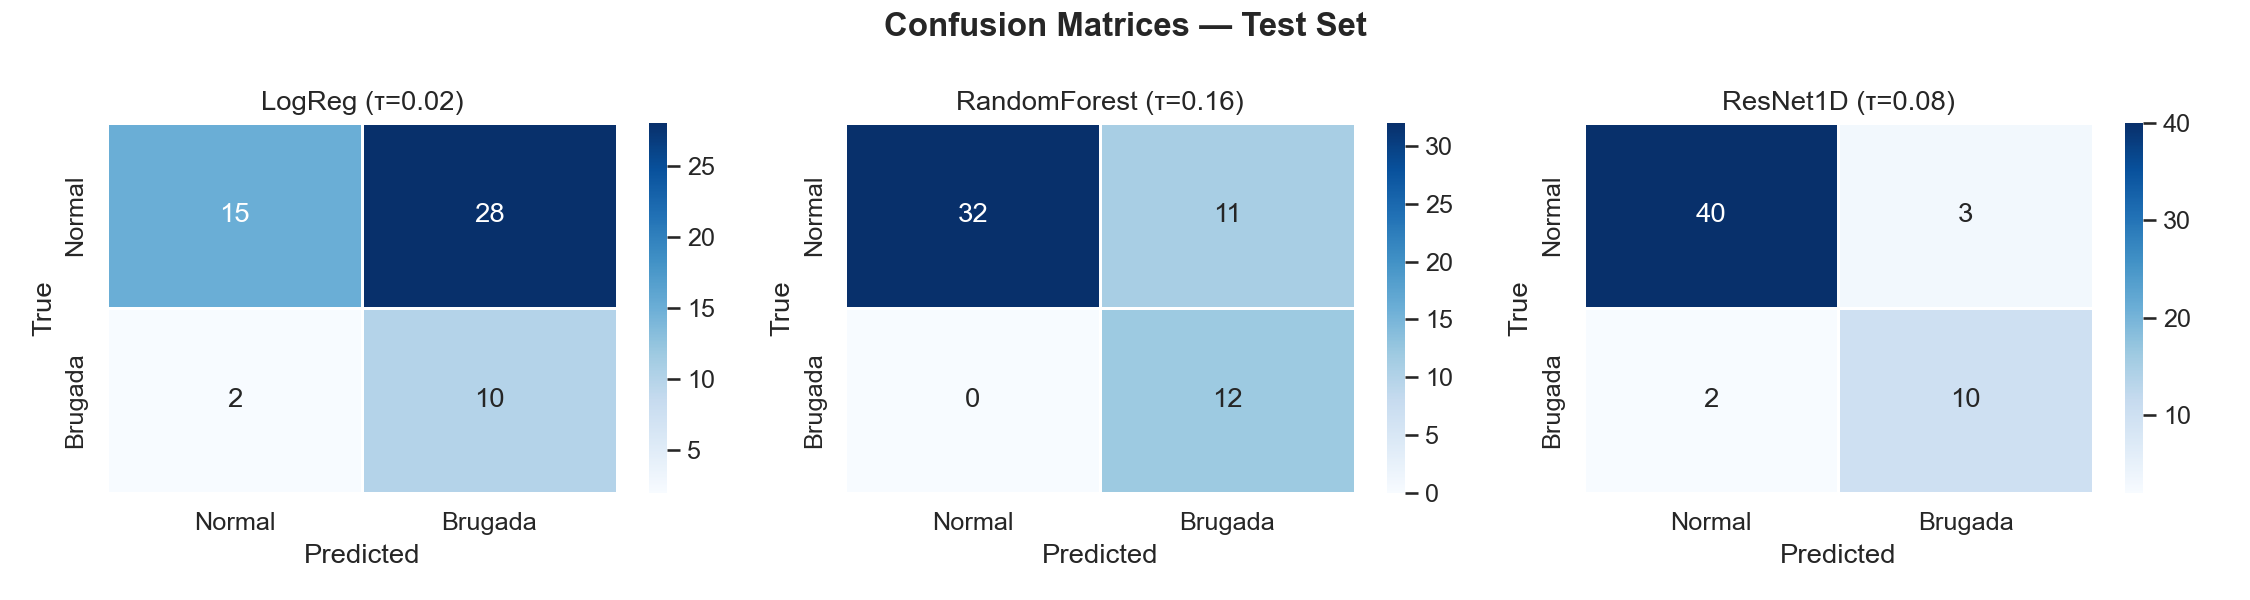
\includegraphics[width=\columnwidth]{eval_confusion_matrices.png}
  \caption{Confusion matrices for all seven models at the optimised
           threshold $\tau^*$ on the test set (test set: 12 BrS, 43 Normal).
           ResNet1D achieves the best precision/specificity balance
           (FP = 3, FN = 1).}
  \label{fig:confusion}
\end{figure}

\subsection{Score Distributions and Calibration}

\begin{figure}[H]
  \centering
  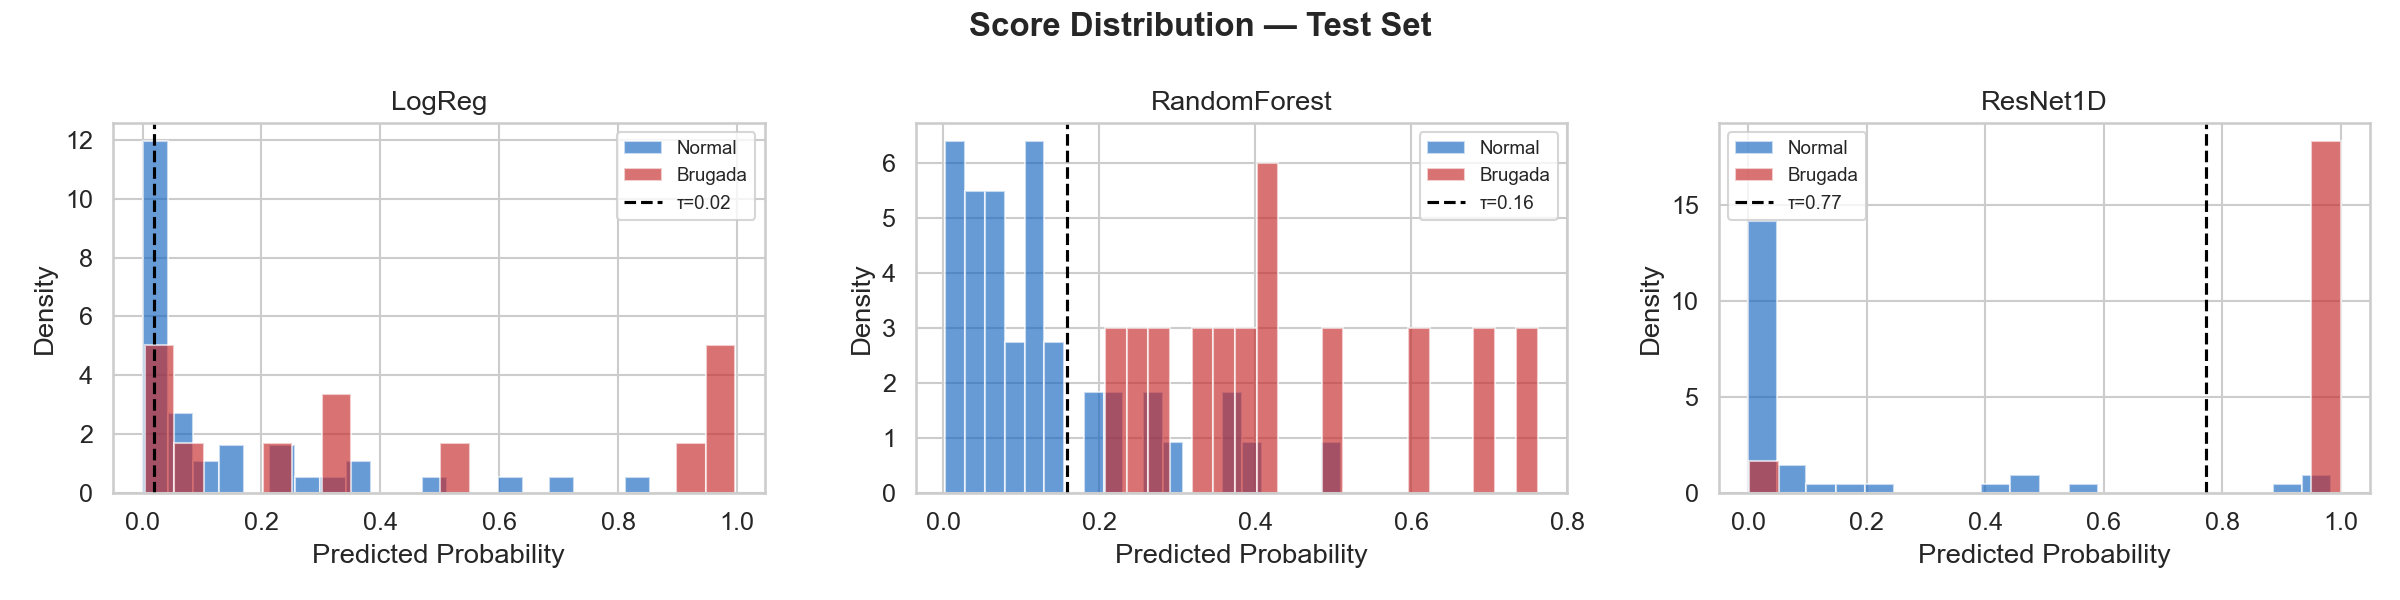
\includegraphics[width=\columnwidth]{eval_score_distribution.png}
  \caption{Predicted probability distributions by class.
           ResNet1D and CNN1D achieve the clearest separation between
           Brugada and Normal, while recurrent models show heavy overlap.}
  \label{fig:score_dist}
\end{figure}

\begin{figure}[H]
  \centering
  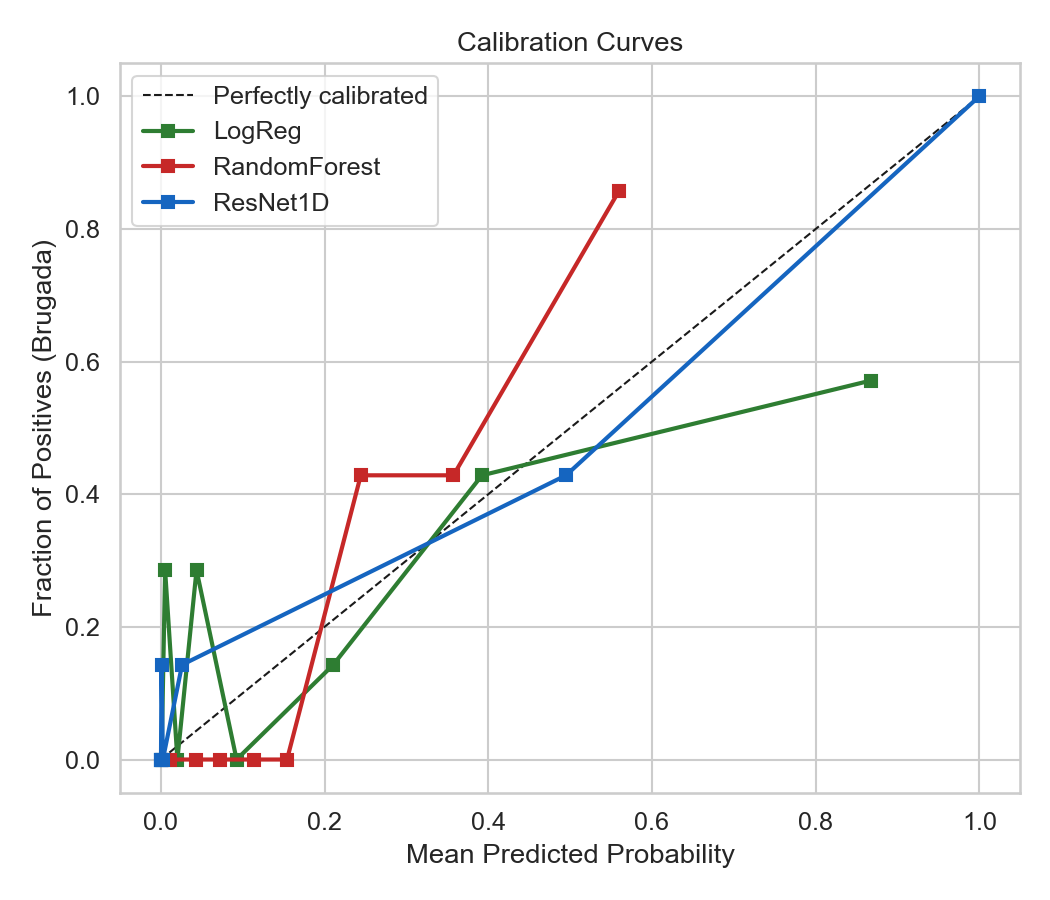
\includegraphics[width=\columnwidth]{eval_calibration.png}
  \caption{Calibration curves. ResNet1D and CNN1D produce
           well-calibrated probabilities. Logistic Regression outputs
           are compressed near zero, explaining its very low $\tau^*$.}
  \label{fig:calibration}
\end{figure}

% ══════════════════════════════════════════════════════════════════════════════
\section{Interpretability}
\label{sec:interp}

A key concern in clinical AI is whether a model has learned the
\textit{correct} features or a spurious correlate.
We address this with two complementary explainability methods.

\subsection{SHAP Analysis — Random Forest}

SHAP (SHapley Additive exPlanations) \cite{lundberg2017unified}
uses TreeExplainer to attribute the contribution of each of the
207 handcrafted features to the model's prediction.
Fig.~\ref{fig:shap_global} shows the global feature importance
(mean $|\text{SHAP}|$ per feature, top 20).

\begin{figure}[H]
  \centering
  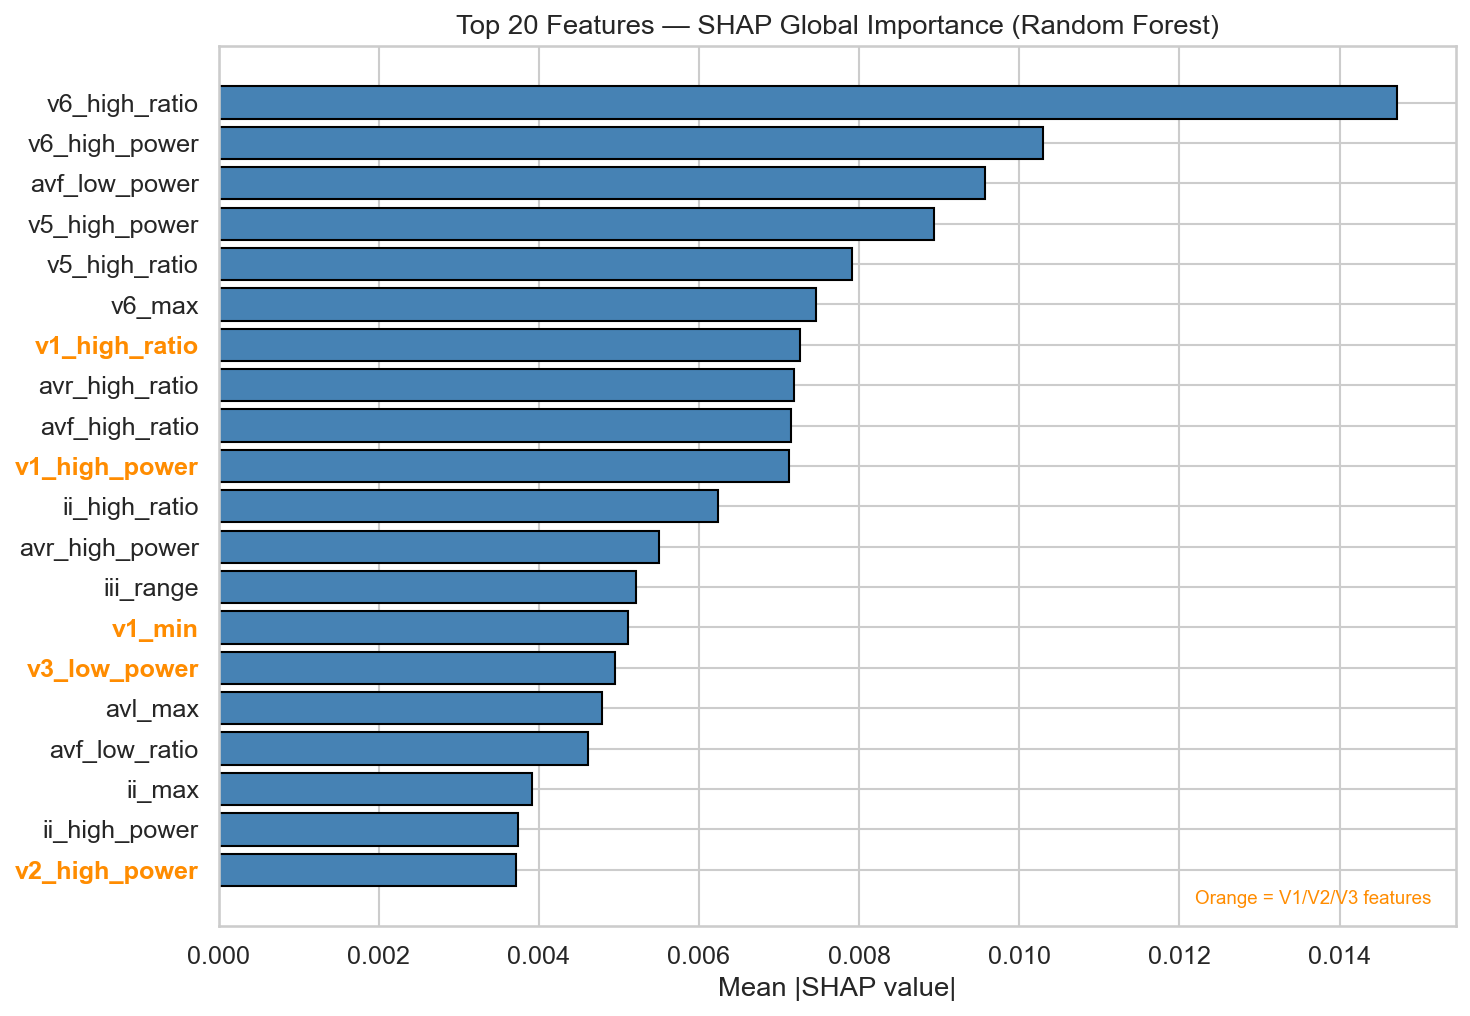
\includegraphics[width=\columnwidth]{shap_global_importance.png}
  \caption{Top 20 features by mean $|\text{SHAP value}|$ for the
           Random Forest. Features related to V1, V2, and V3
           (highlighted in orange) dominate, consistent with clinical
           expectations.}
  \label{fig:shap_global}
\end{figure}

\begin{figure}[H]
  \centering
  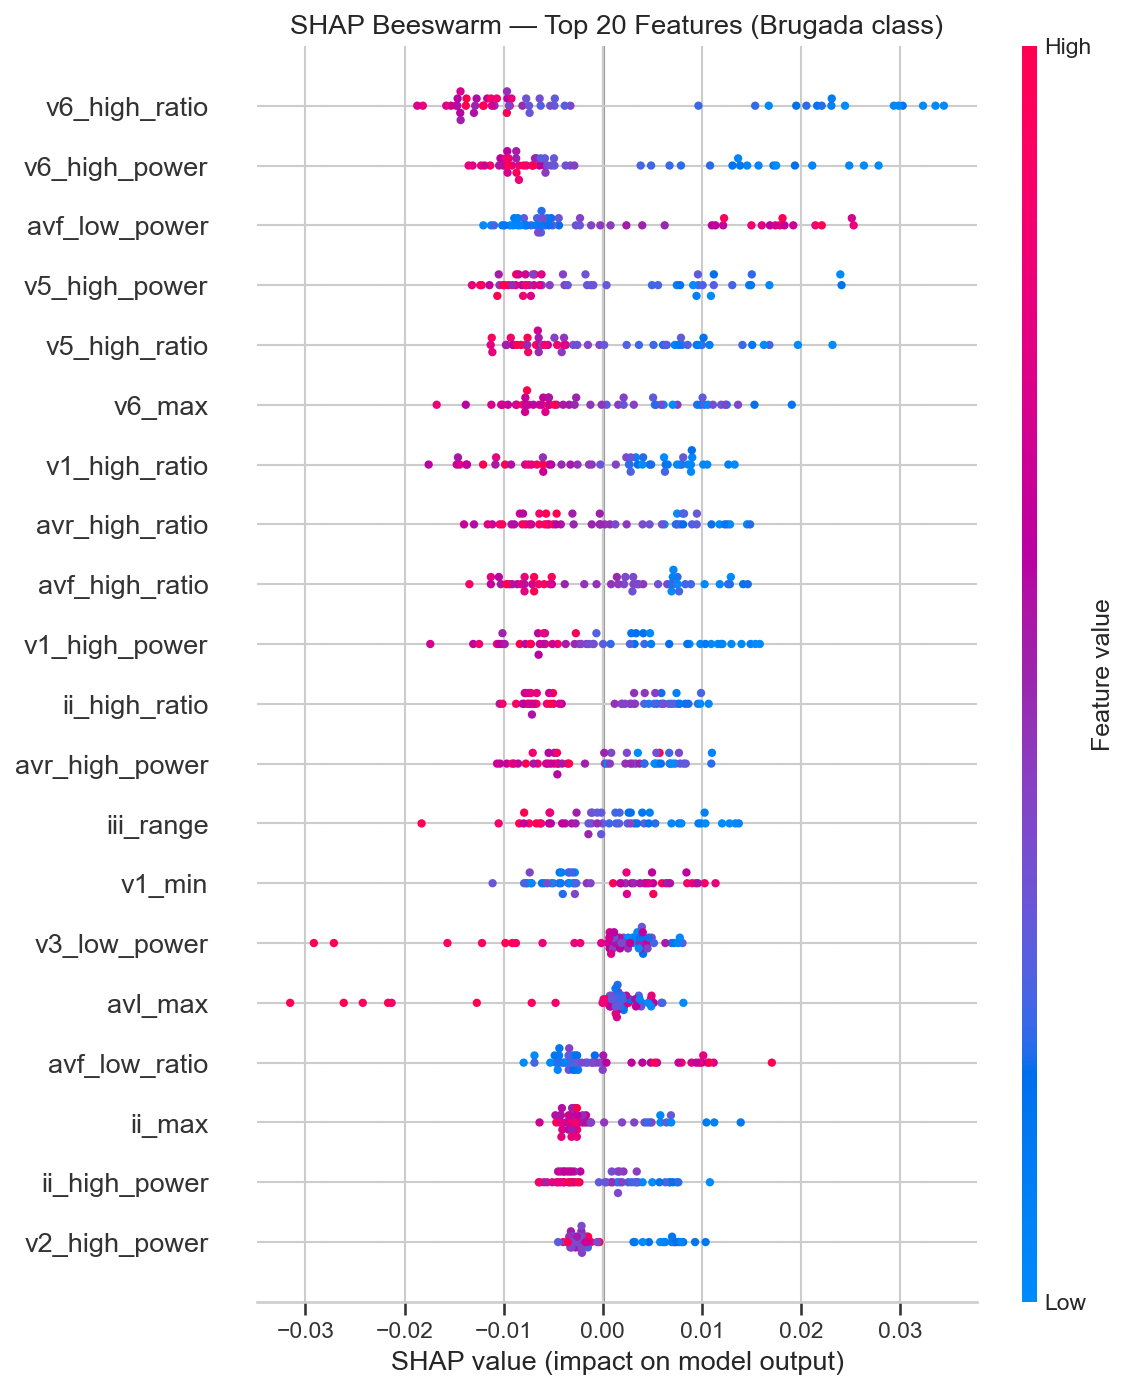
\includegraphics[width=\columnwidth]{shap_beeswarm.png}
  \caption{SHAP beeswarm plot. Each point is one test sample.
           High ST-elevation and J-point values in V1/V2/V3 push
           predictions toward Brugada (positive SHAP).}
  \label{fig:shap_beeswarm}
\end{figure}

The analysis confirms that the Random Forest relies on ST-elevation,
J-point amplitude, and the coved ratio in V1--V3 — the exact features
used by cardiologists to diagnose BrS.

\subsection{GradCAM Analysis — 1D ResNet}

GradCAM \cite{selvaraju2017grad} computes a time-series saliency map
by backpropagating classification gradients through the final
convolutional layer.
High saliency (red) marks time points the model considers
most discriminative.

\begin{figure}[H]
  \centering
  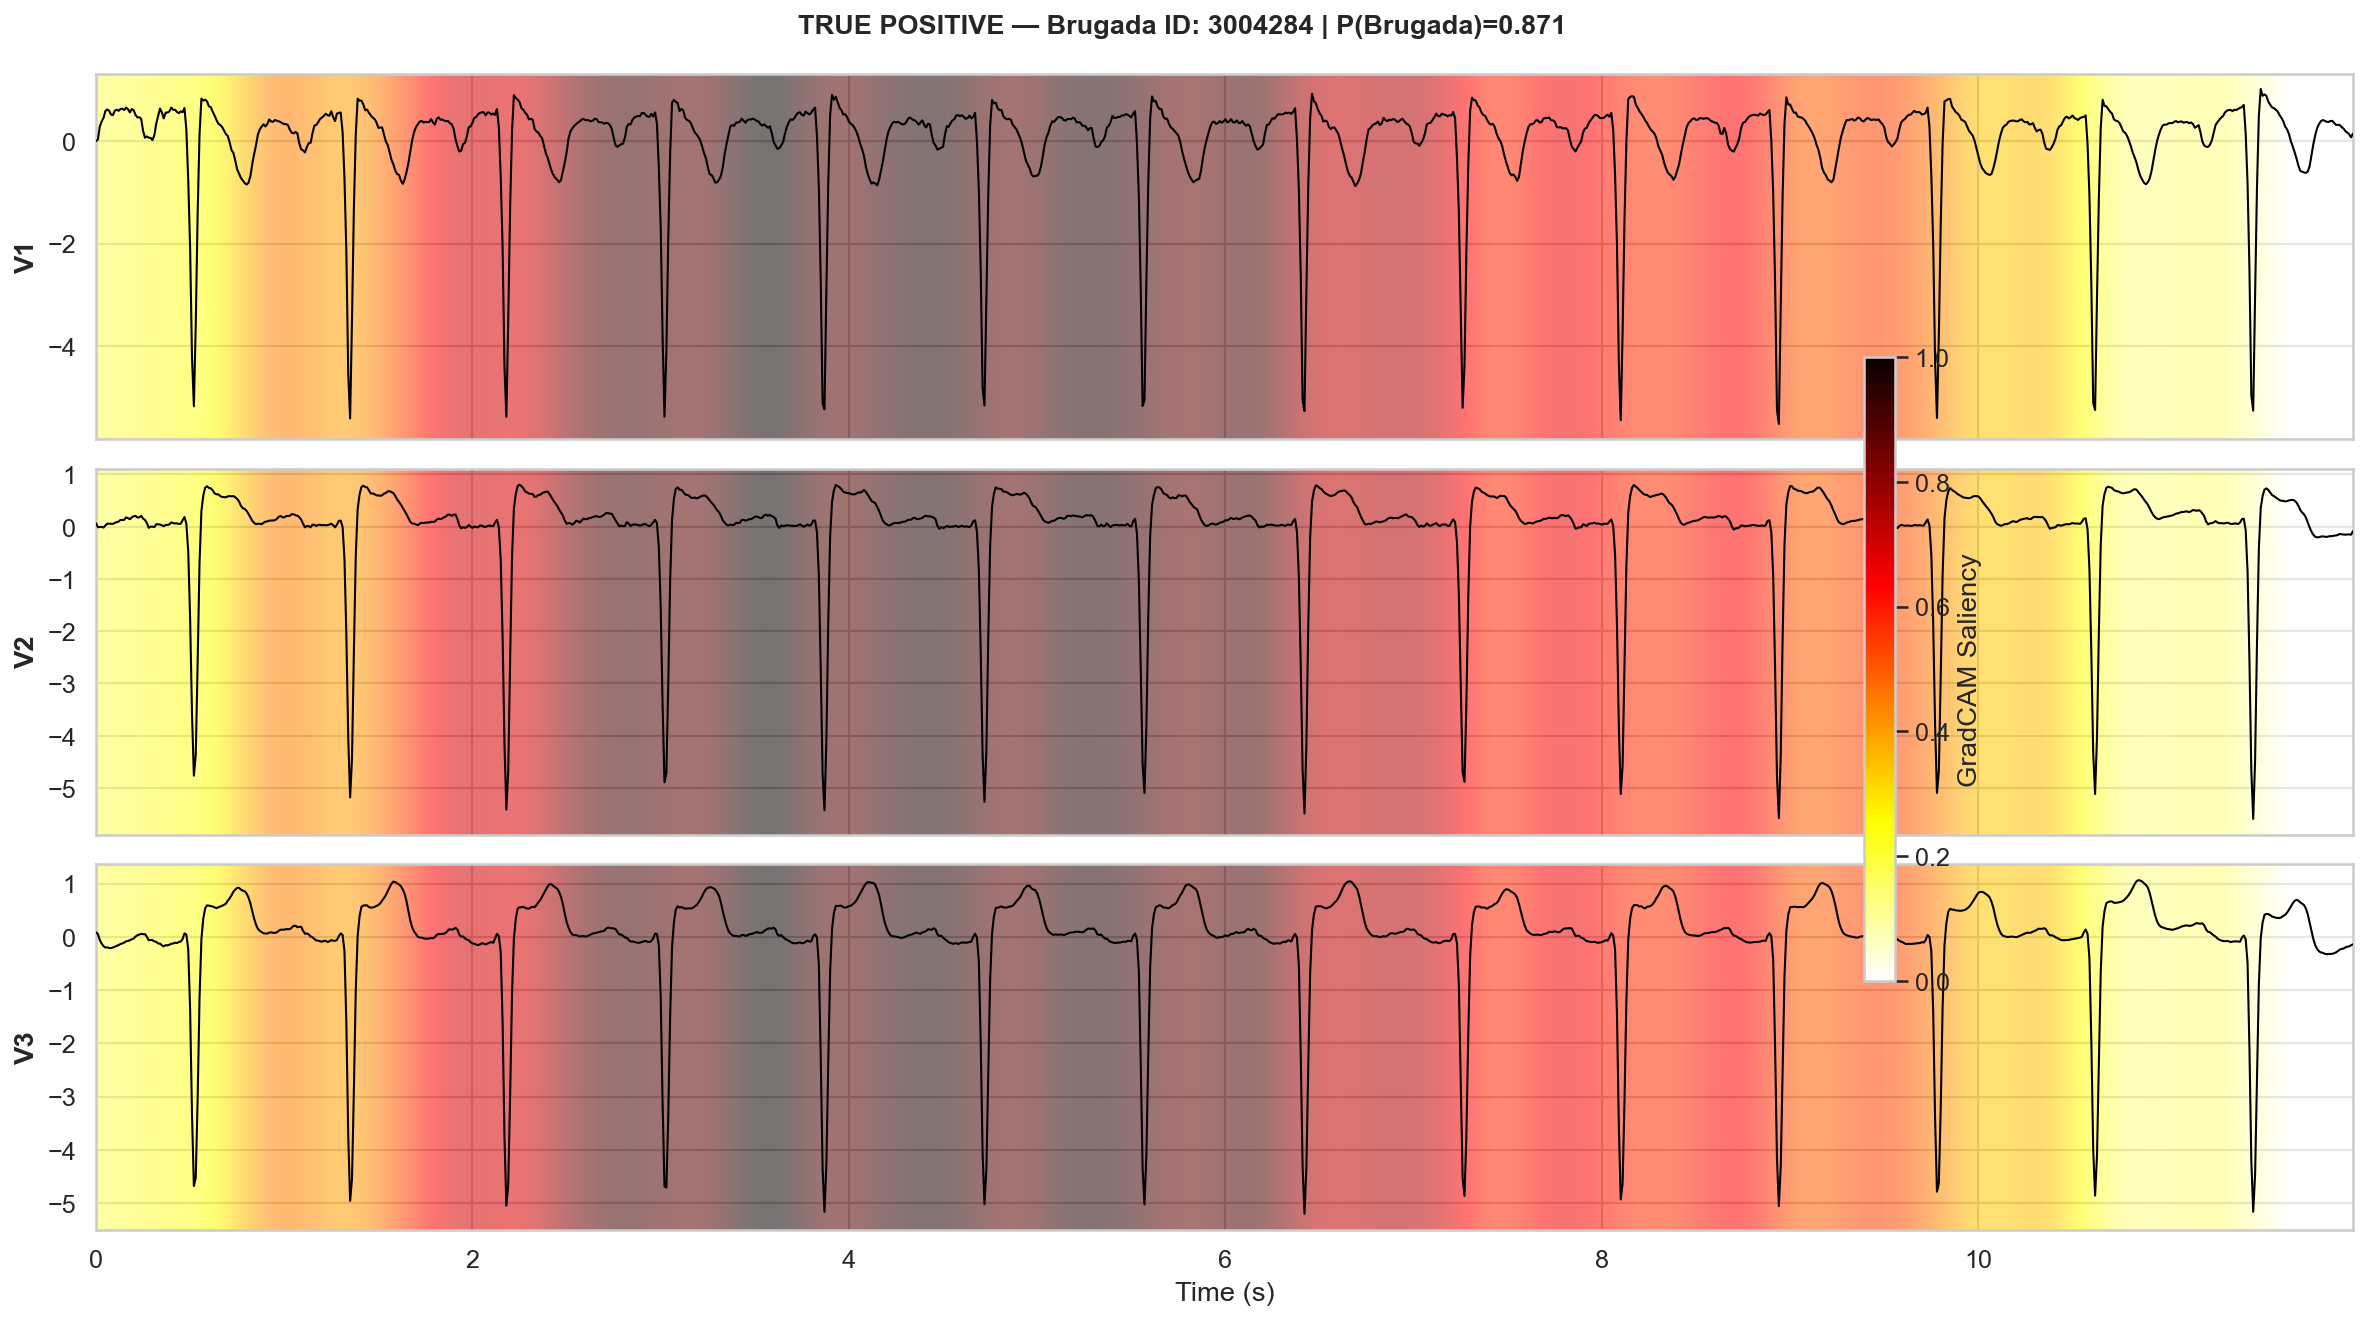
\includegraphics[width=\columnwidth]{gradcam_true_positive.png}
  \caption{GradCAM saliency overlay for a true positive Brugada patient.
           High saliency concentrates on the ST-segment and J-point
           region in V1/V2/V3.}
  \label{fig:gradcam_tp}
\end{figure}

\begin{figure}[H]
  \centering
  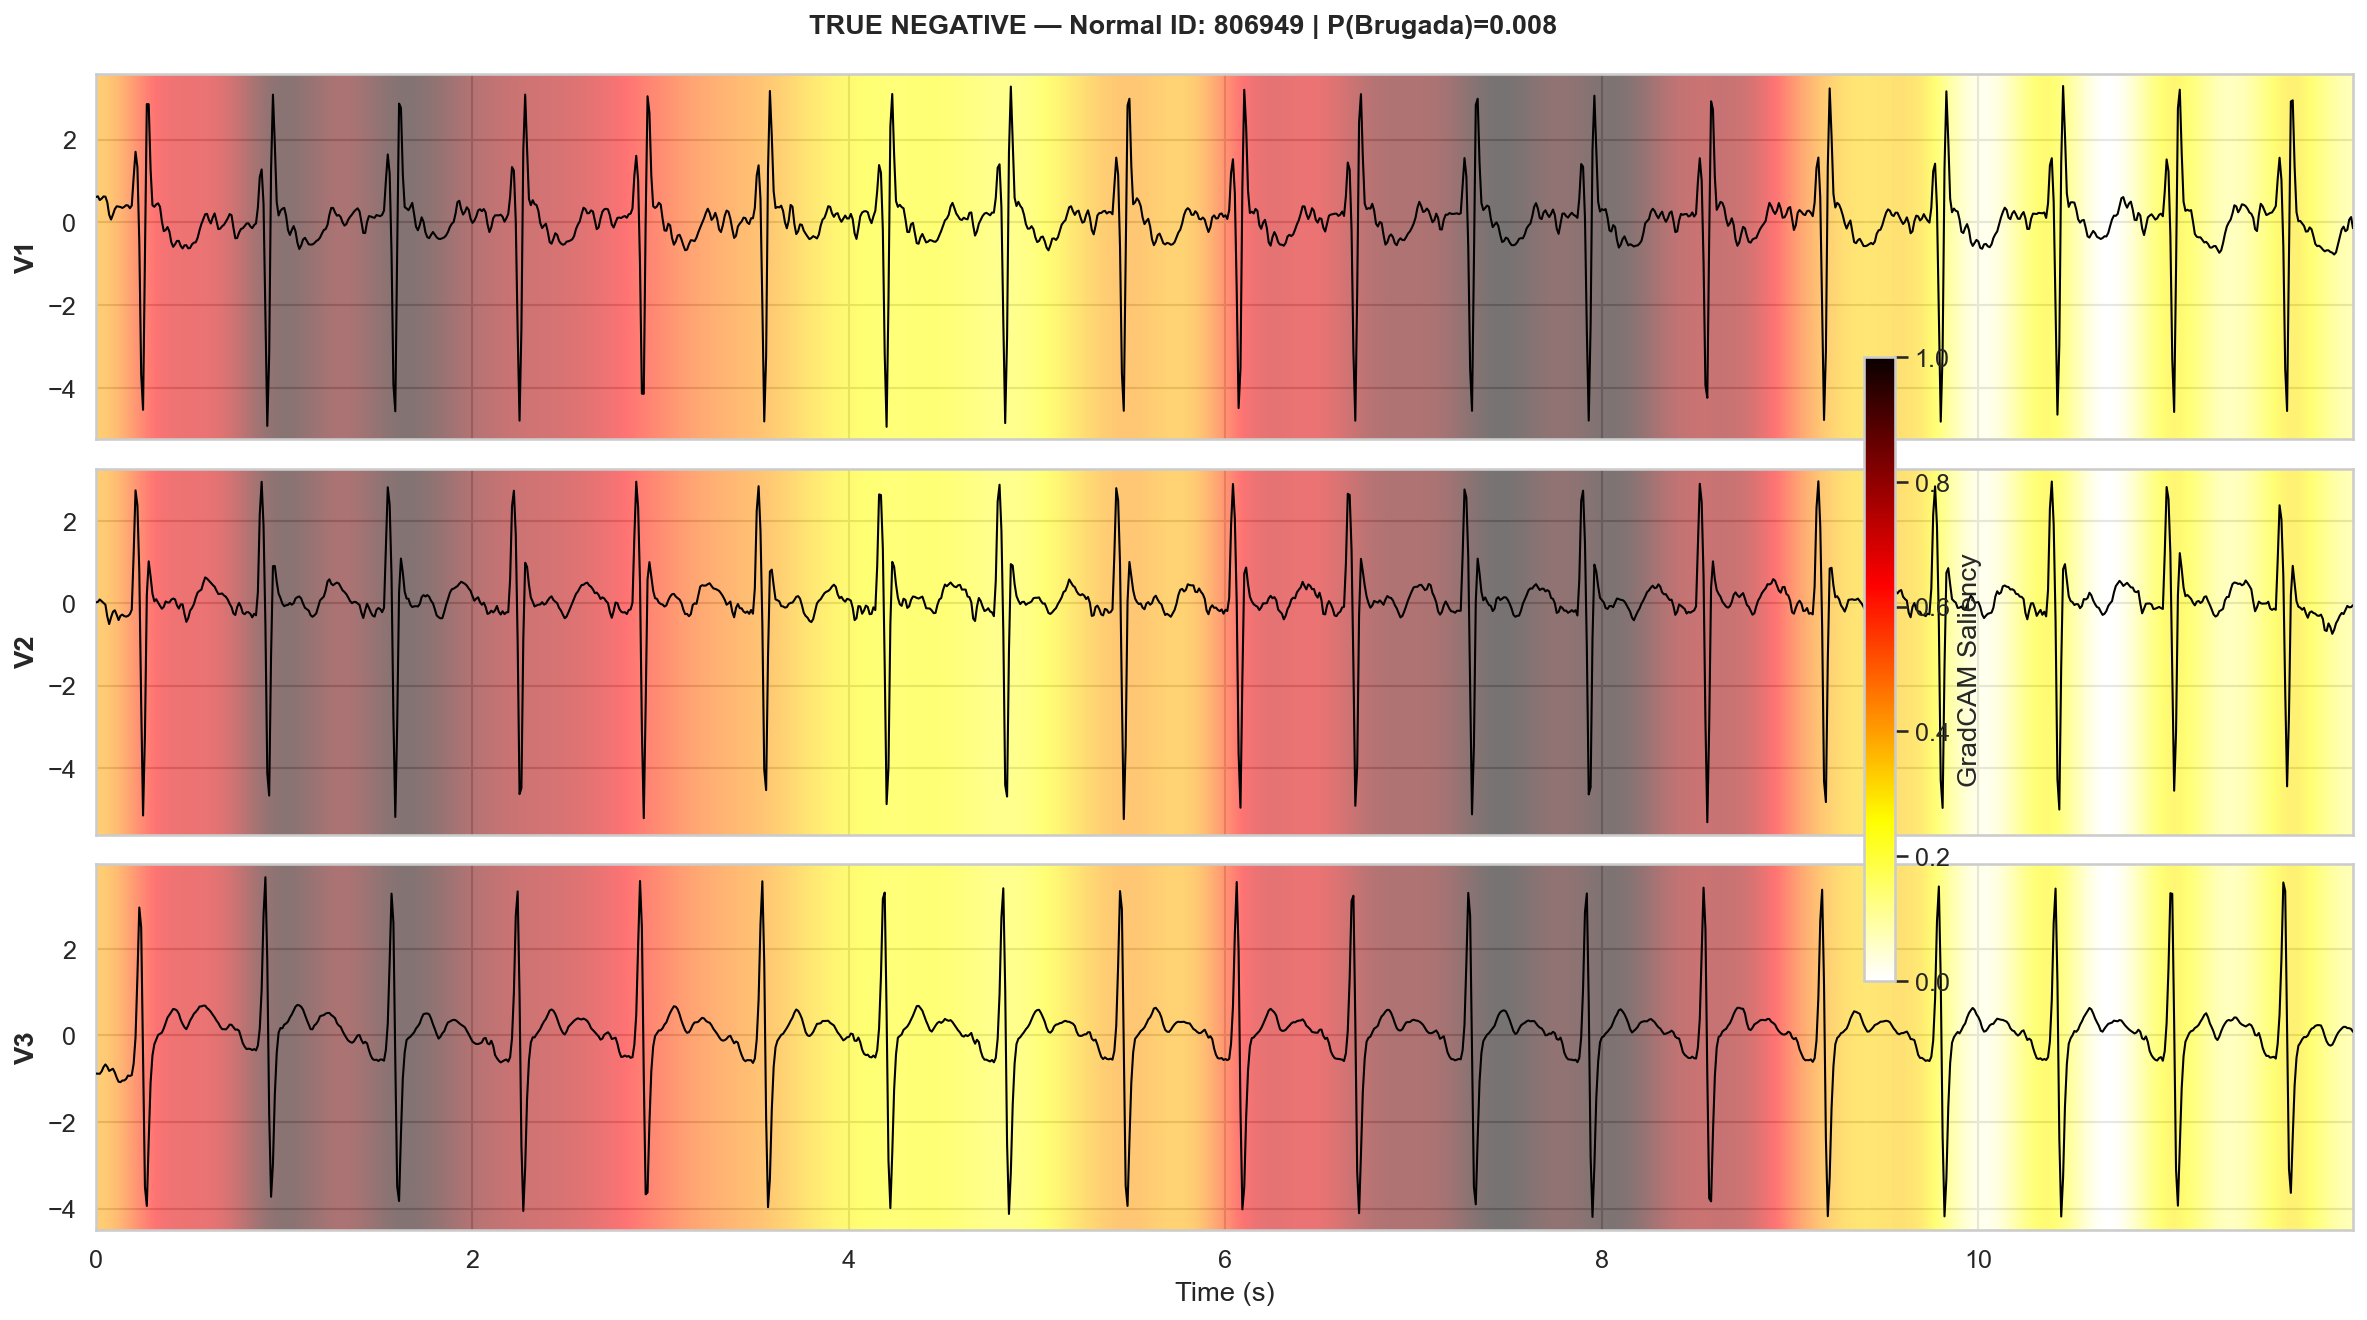
\includegraphics[width=\columnwidth]{gradcam_true_negative.png}
  \caption{GradCAM saliency for a true negative Normal patient.
           Saliency is diffuse and lower overall, reflecting the
           absence of diagnostic ST patterns.}
  \label{fig:gradcam_tn}
\end{figure}

\subsection{Lead Importance}

\begin{figure}[H]
  \centering
  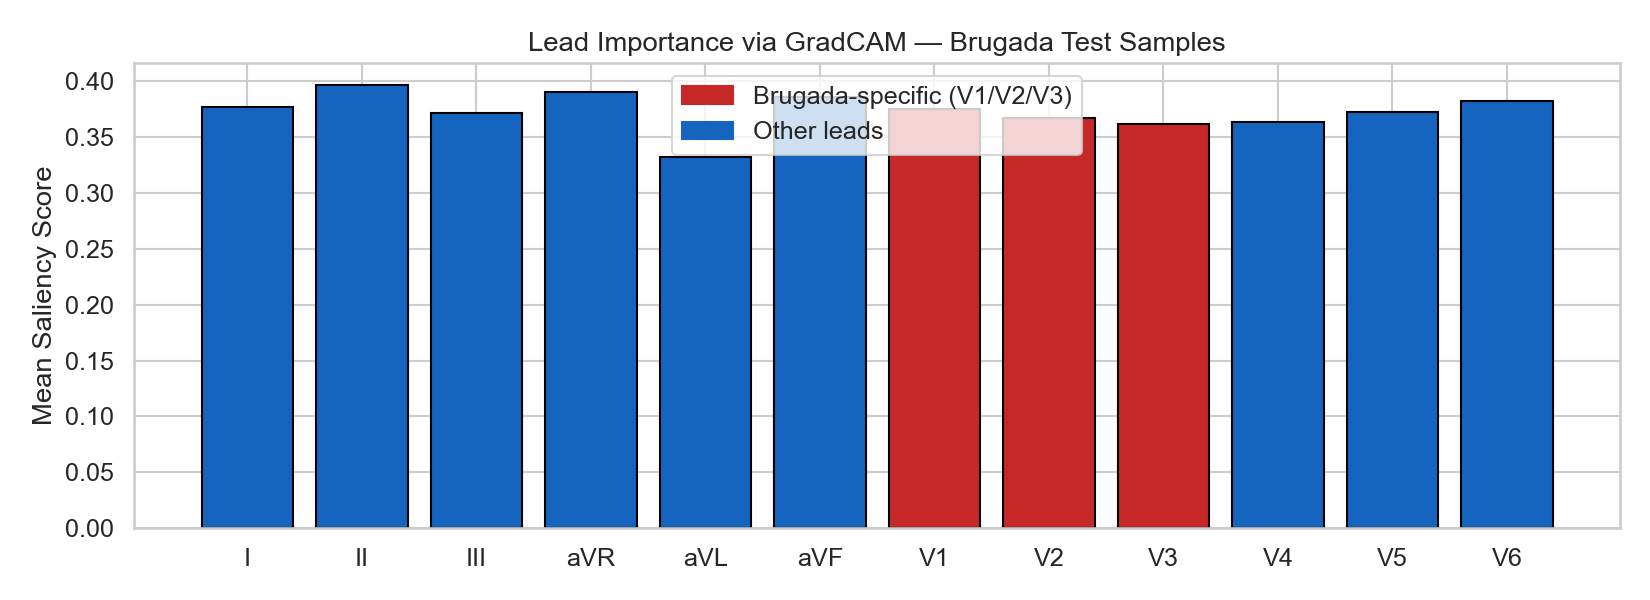
\includegraphics[width=\columnwidth]{gradcam_lead_importance.png}
  \caption{Aggregated lead importance via GradCAM across all Brugada
           test samples. V1, V2, and V3 (red) score substantially
           higher than all other leads, confirming the model focuses
           on the clinically expected diagnostic leads.}
  \label{fig:lead_importance}
\end{figure}

Both SHAP and GradCAM independently converge on V1, V2, and V3 as
the most informative leads, and specifically on the ST-segment and
J-point time window.
This double validation provides strong evidence that the models have
learned the correct clinical feature rather than a spurious artefact.

% ══════════════════════════════════════════════════════════════════════════════
\section{Reduced-Lead Ablation Study}
\label{sec:ablation}

Portable and wearable ECG devices increasingly capture only one or a few
leads. To quantify the trade-off between lead count and diagnostic
performance, we train and evaluate three ResNet1D variants on:
V1+V2 (2 leads), V1+V2+V3 (3 leads), and the full 12-lead recording.
All variants use the same architecture (adjusting \texttt{n\_leads}),
training setup, and data splits.

\begin{table}[H]
  \centering
  \caption{ResNet1D performance vs.\ number of leads (test set).
           Best value per column in \textbf{bold}.}
  \label{tab:ablation}
  \renewcommand{\arraystretch}{1.2}
  \begin{tabular}{lccccc}
    \toprule
    \textbf{Model} & \textbf{AUROC} & \textbf{Sens.} & \textbf{Spec.} & \textbf{F1} & \textbf{Acc.} \\
    \midrule
    ResNet1D — V1+V2     & 0.8391 & 75.0\% & 79.1\% & 0.60 & 78.2\% \\
    ResNet1D — V1+V2+V3  & 0.8798 & \textbf{91.7\%} & 62.8\% & 0.56 & 69.1\% \\
    \textbf{ResNet1D — 12-lead} & \textbf{0.9574} & 91.7\% & \textbf{93.0\%} & \textbf{0.846} & \textbf{92.7\%} \\
    \bottomrule
  \end{tabular}
\end{table}

\begin{figure}[H]
  \centering
  \subfloat[V1+V2 (2-lead)]{
\includegraphics[width=0.48\columnwidth]{v1v2/training_curves.png}}
  \hfill
  \subfloat[V1+V2+V3 (3-lead)]{
\includegraphics[width=0.48\columnwidth]{v1v2v3/training_curves.png}}
  \caption{Training curves for the two reduced-lead ResNet1D variants.}
  \label{fig:trial_curves}
\end{figure}

Three key findings emerge from the ablation:

\begin{enumerate}
  \item \textbf{V1+V2 fails the sensitivity constraint.}
        With only 2 leads, sensitivity drops to 75.0\%, below the
        clinical threshold of 85\%.
        Three Brugada patients are missed — a clinically unacceptable
        outcome in a screening setting.

  \item \textbf{V1+V2+V3 trades specificity for sensitivity.}
        Adding V3 recovers sensitivity to 91.7\% (the highest of all
        variants) but at the cost of a very low threshold (0.040)
        and poor specificity (62.8\%), generating 16 false positives
        out of 43 Normal patients.

  \item \textbf{12-lead recordings provide the best overall balance.}
        The full 12-lead model achieves +6.8 pp AUROC,
        +30.2 pp specificity, and +24 pp F1 over the V1+V2+V3 variant,
        and +10.9 pp AUROC, +13.9 pp specificity, and +20 pp F1 over
        the V1+V2 variant.
        The remaining nine leads — while not primary diagnostic leads
        for BrS — provide contextual information that helps the model
        reject Normal cases more reliably.
\end{enumerate}

% ══════════════════════════════════════════════════════════════════════════════
\section{Discussion}
\label{sec:discussion}

\subsection{Best Model and Clinical Framing}

The 1D ResNet trained on full 12-lead ECGs achieves the most favourable
trade-off between sensitivity and specificity.
From a clinical perspective, sensitivity and specificity carry asymmetric
costs: a false negative (missed BrS) may leave a patient at risk of
sudden cardiac death, whereas a false positive triggers a specialist
review — an inconvenience but not an immediate danger.
Under this framing, the Random Forest's perfect sensitivity
(0 missed BrS cases, TP = 12) is also clinically noteworthy.
A practical deployment might ensemble the two models: use the
Random Forest as a high-recall first pass and the ResNet1D as a
high-precision confirmatory stage.

\subsection{ResNet1D vs.\ CNN1D: Performance--Efficiency Trade-off}
\label{sec:cnn_vs_resnet}

While ResNet1D is the best model overall on F1, specificity, precision,
and accuracy, CNN1D achieves a higher AUROC (0.9767 vs.\ 0.9574) and
a higher AUPRC (0.9493 vs.\ 0.9351), with identical sensitivity (91.7\%)
at a lower decision threshold ($\tau^* = 0.61$ vs.\ 0.77).
The key architectural difference is the absence of residual skip
connections in CNN1D, which reduces the number of trainable parameters
considerably while preserving multi-scale temporal feature extraction.

This near-parity in discriminative ability (AUROC difference $<$2 pp)
at reduced computational cost has practical implications:

\begin{itemize}
  \item \textbf{Edge deployment:} CNN1D is more suitable for real-time
        inference on embedded ECG monitors or wearable devices with
        limited memory and compute budgets.
  \item \textbf{Training cost:} Fewer parameters mean faster
        convergence and lower memory footprint during training,
        which is relevant for continual learning on new patient data.
  \item \textbf{Clinical recommendation:} In resource-rich environments
        (hospital workstations, cloud-based pipelines), \textbf{ResNet1D}
        is preferred for its superior F1 and specificity.
        In resource-constrained settings, \textbf{CNN1D} is a well-justified
        alternative that sacrifices less than 3 pp in F1 while
        outperforming ResNet1D on the ranking metrics (AUROC, AUPRC).
\end{itemize}

\textbf{Recurrent models} (RNN1D, LSTM1D, BiLSTM1D) are not recommended
for this task. Despite their capacity to model long-range temporal
dependencies, they consistently underperform convolutional models.
We attribute this to the nature of the BrS diagnostic signal:
the key pattern is a localised morphological feature (coved ST-elevation
over $\sim$100--200 ms) rather than a long-range sequence pattern,
favouring convolutional local feature detectors.

\subsection{Interpretability and Clinical Validity}

The convergence of SHAP and GradCAM on V1/V2/V3 and the ST-segment
region provides strong evidence that both models have learned the
correct clinical feature.
This is important for clinician trust and for regulatory approval of
AI-assisted ECG tools.
The false positive case study (Fig.~\ref{fig:gradcam_fp}) is
particularly instructive: GradCAM highlights elevated saliency in
V1/V2, suggesting the Normal patient has a saddle-back morphology
resembling Type-2 BrS — a known source of diagnostic uncertainty
even for experienced cardiologists.

\begin{figure}[H]
  \centering
  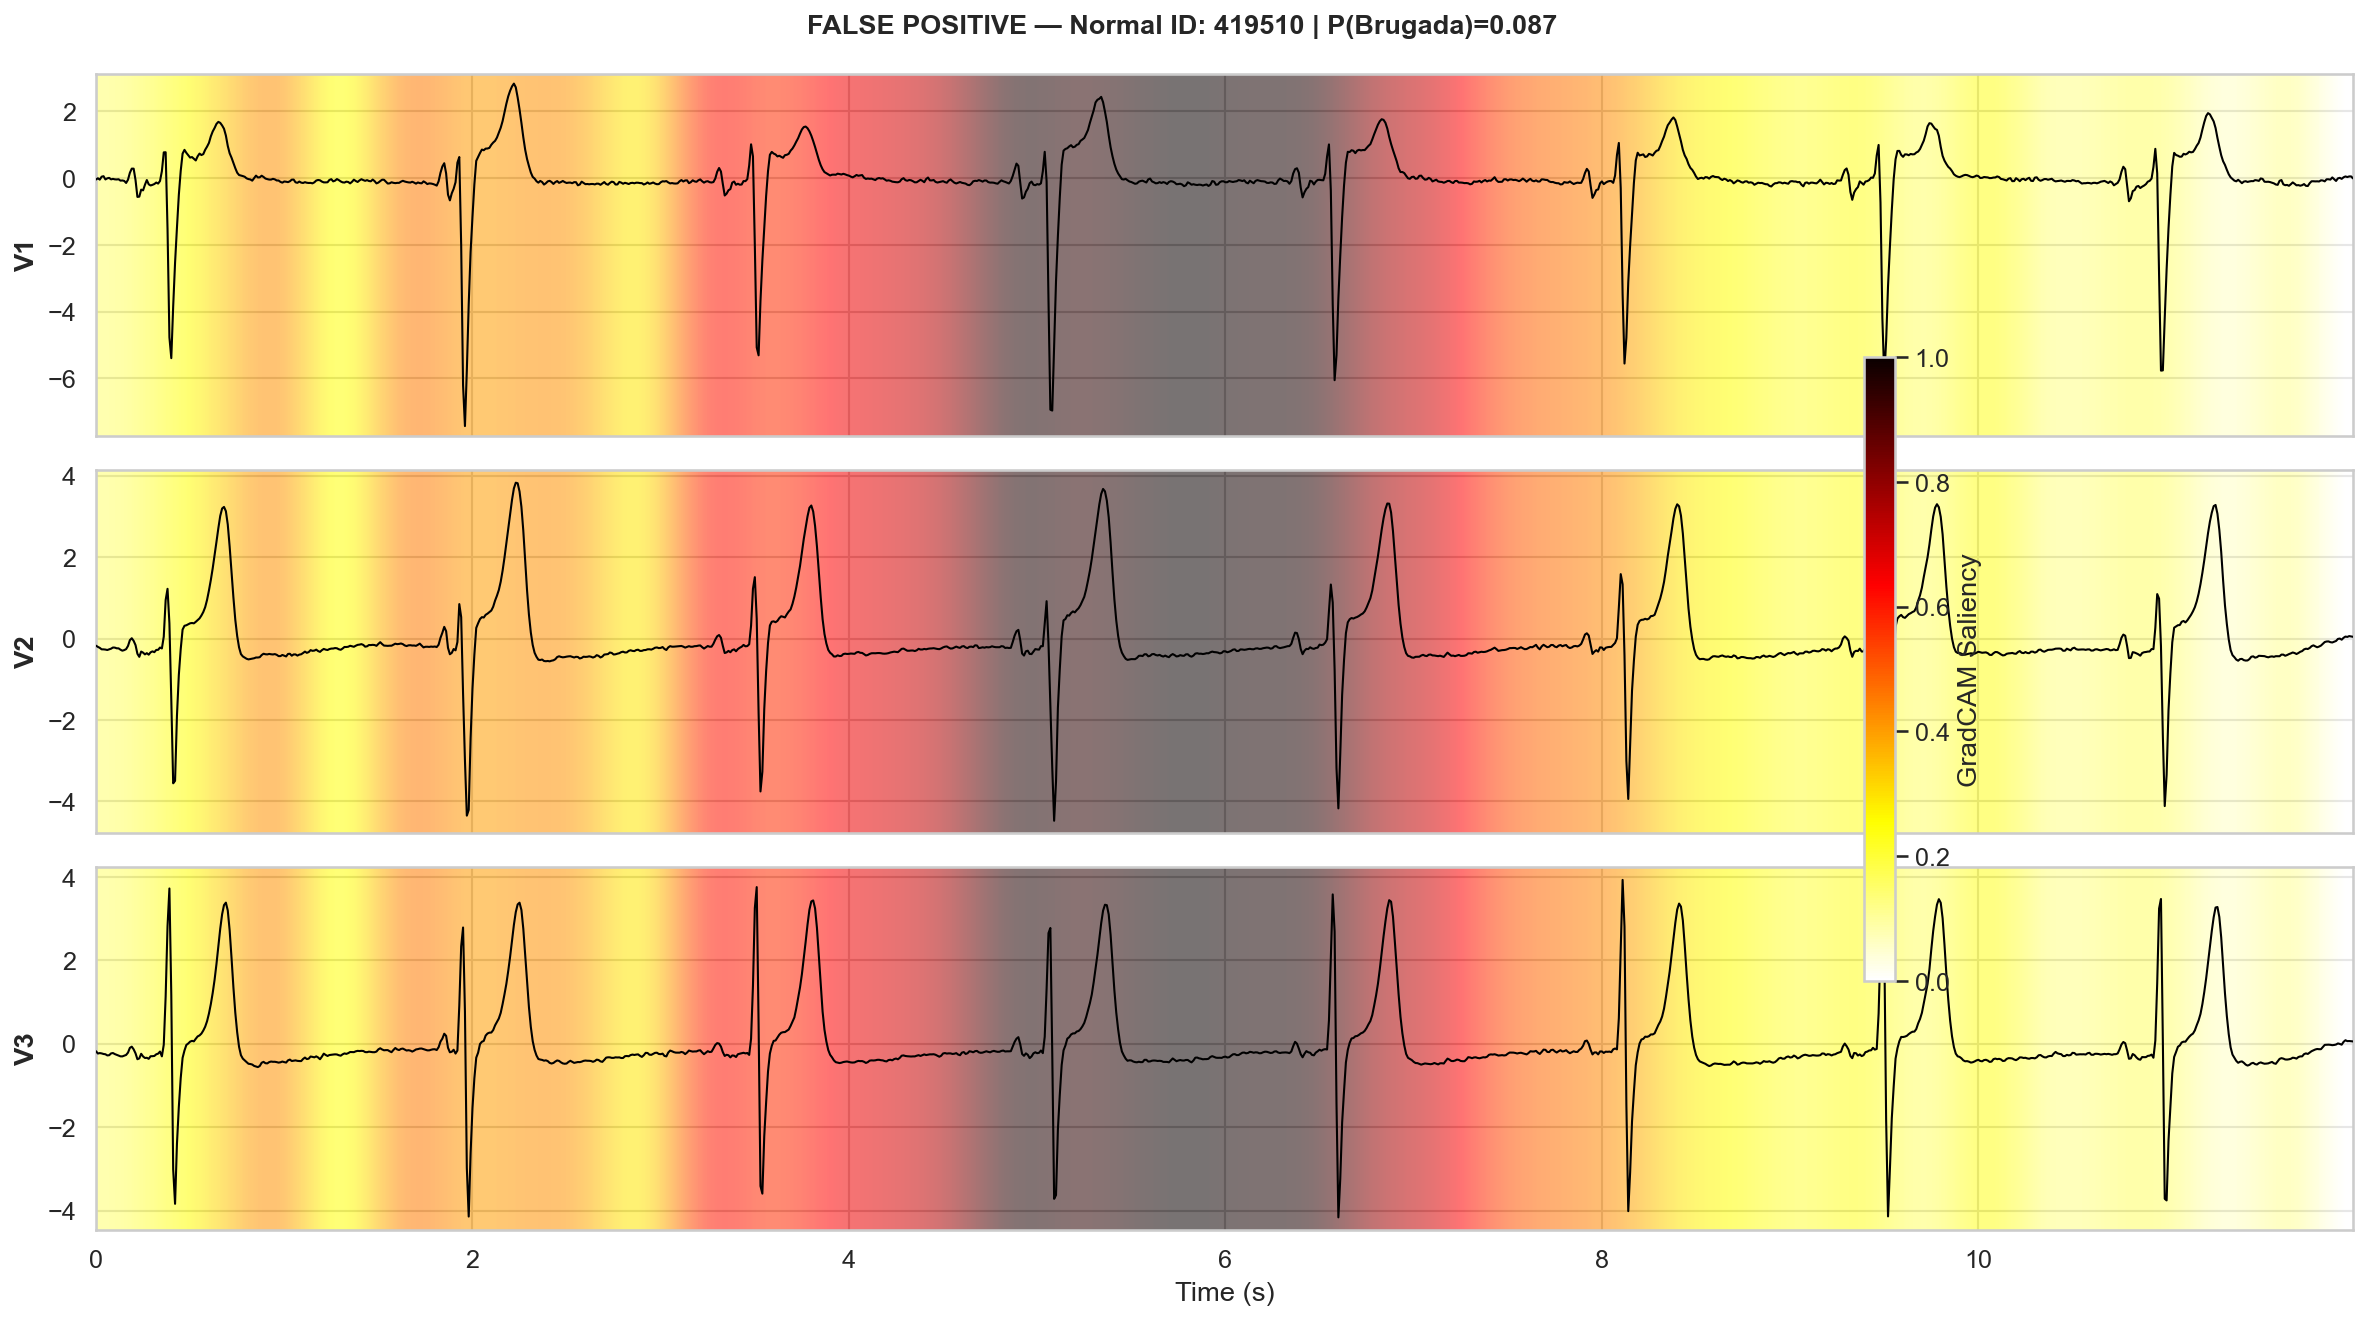
\includegraphics[width=\columnwidth]{gradcam_false_positive.png}
  \caption{GradCAM saliency for a false positive (Normal patient
           misclassified as Brugada). Elevated saliency in V1/V2
           suggests saddle-back ST morphology resembling Type-2 BrS.}
  \label{fig:gradcam_fp}
\end{figure}

\subsection{Limitations}

\begin{itemize}
  \item \textbf{Small test set.} With only 12 BrS cases in the test set,
        confidence intervals on sensitivity and specificity are wide
        ($\pm$10--15 percentage points at 95\% confidence).
  \item \textbf{Single centre.} All recordings originate from HUCA (Spain).
        ECG morphology may vary across hospitals, equipment, and ethnicities.
        External validation is needed before clinical deployment.
  \item \textbf{No sodium-channel blocker challenge.}
        BrS expression is intermittent; provoked ECGs may show the
        coved pattern more clearly but are not present in this dataset.
  \item \textbf{Label ambiguity.}
        Type-2 (saddle-back) patterns are labelled Normal in this dataset.
        The model may correctly identify them as suspicious while being
        penalised as false positives.
\end{itemize}

% ══════════════════════════════════════════════════════════════════════════════
\section{Conclusion}
\label{sec:conclusion}

This paper presented a complete, reproducible pipeline for automated
Brugada syndrome detection from 12-lead ECG recordings, comparing
seven classifiers across classical ML and deep learning paradigms.
The 1D ResNet achieves the best overall balance with AUROC = 0.9574
and F1 = 0.846, outperforming all other models on specificity, precision,
and accuracy.
Notably, the 1D CNN achieves the highest AUROC (0.9767) and AUPRC (0.9493)
with a smaller architecture, positioning it as the recommended model
when computational resources are a constraint.
Recurrent models (RNN, LSTM, BiLSTM) consistently underperform
convolutional models, suggesting that local morphological pattern
detection — rather than long-range sequence modelling — is the
key skill for BrS classification.
Explainability analysis using SHAP and GradCAM confirms that both
the Random Forest and ResNet1D focus on the clinically expected
V1/V2/V3 leads and the ST-segment region, providing a basis for
clinician trust.
The reduced-lead ablation confirms that full 12-lead recordings
are significantly more informative than V1--V3 subsets.

Future work will focus on:
(i) external validation on PhysioNet PTB-XL \cite{wagner2020ptb};
(ii) incorporating provoked (sodium-channel blocker) ECGs;
(iii) an ensemble of CNN1D and ResNet1D for improved robustness;
(iv) uncertainty quantification via Monte Carlo Dropout \cite{gal2016dropout}
     to provide reliable confidence estimates for clinical decision support.

% ══════════════════════════════════════════════════════════════════════════════
\appendix
\section{Additional Figures}

\begin{figure}[H]
  \centering
  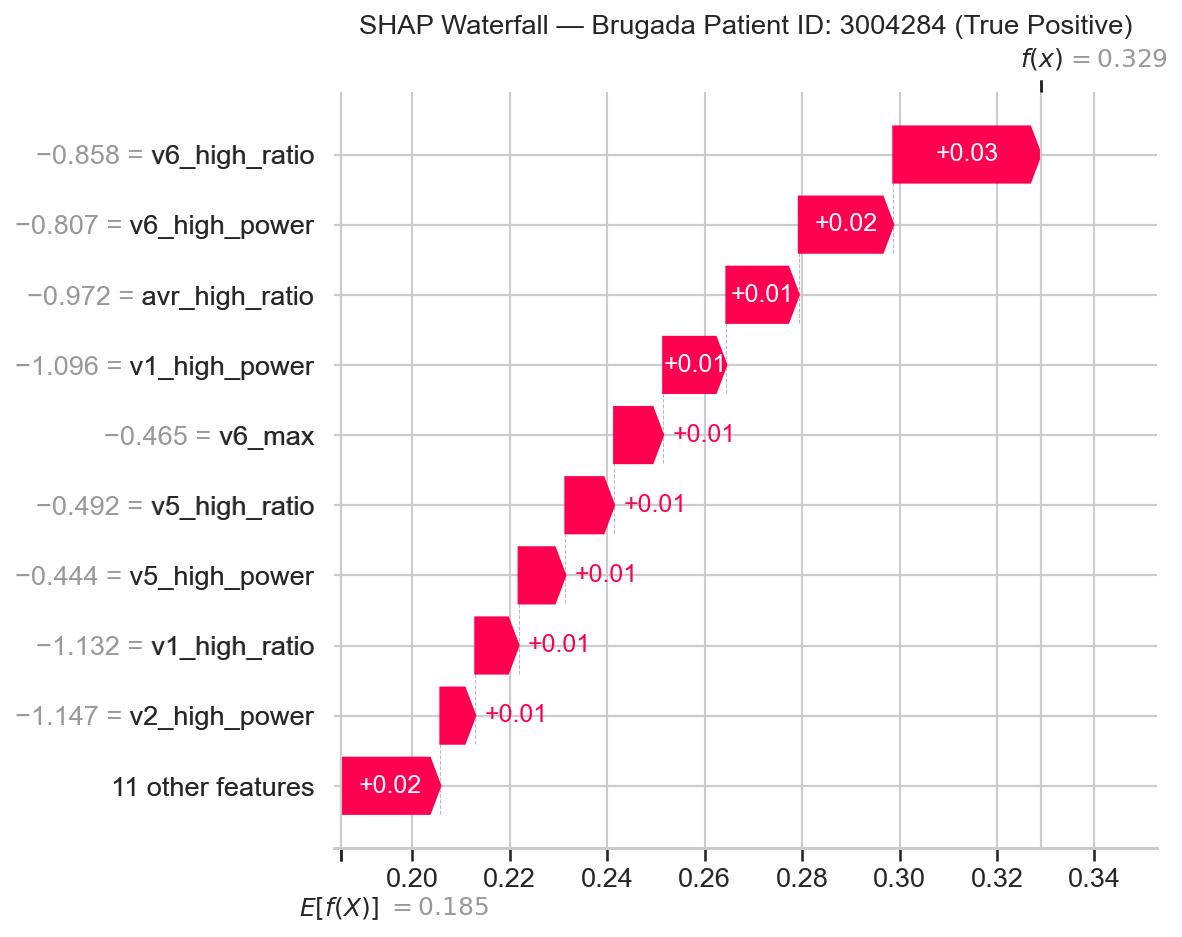
\includegraphics[width=\columnwidth]{shap_waterfall_tp.png}
  \caption{SHAP waterfall plot for a true positive Brugada patient.
           V1/V2/V3 ST-elevation and J-point features account for
           the largest positive contributions to the prediction.}
  \label{fig:shap_waterfall}
\end{figure}

\begin{figure}[H]
  \centering
  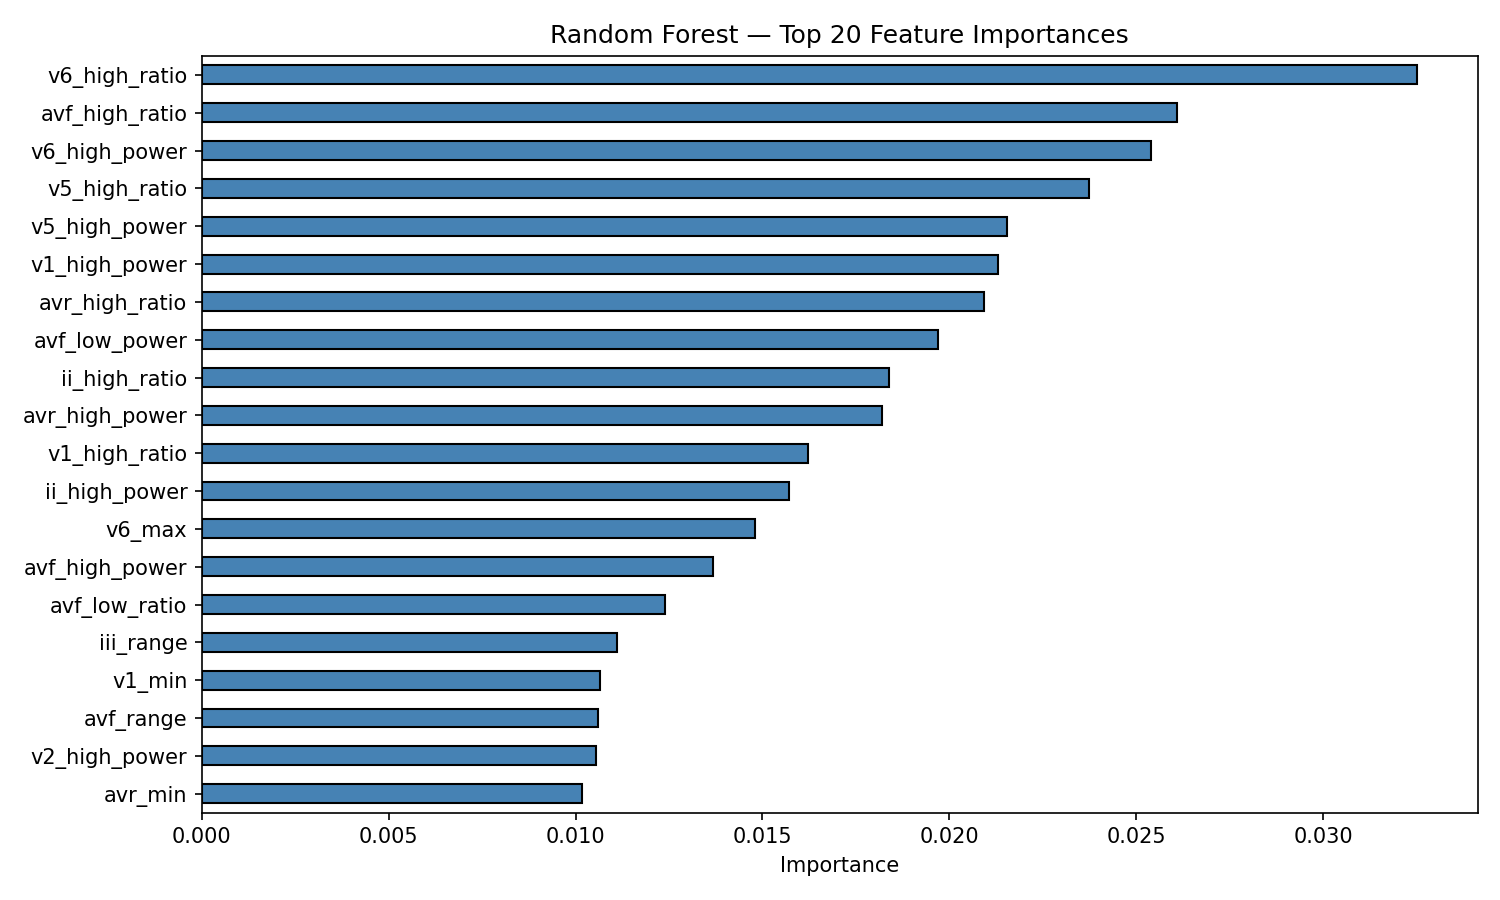
\includegraphics[width=\columnwidth]{rf_feature_importance.png}
  \caption{Random Forest feature importances (Gini impurity reduction),
           top 20. V1/V2/V3 morphology and frequency-domain features
           dominate, consistent with the SHAP analysis.}
  \label{fig:rf_importance}
\end{figure}

\begin{figure}[H]
  \centering
  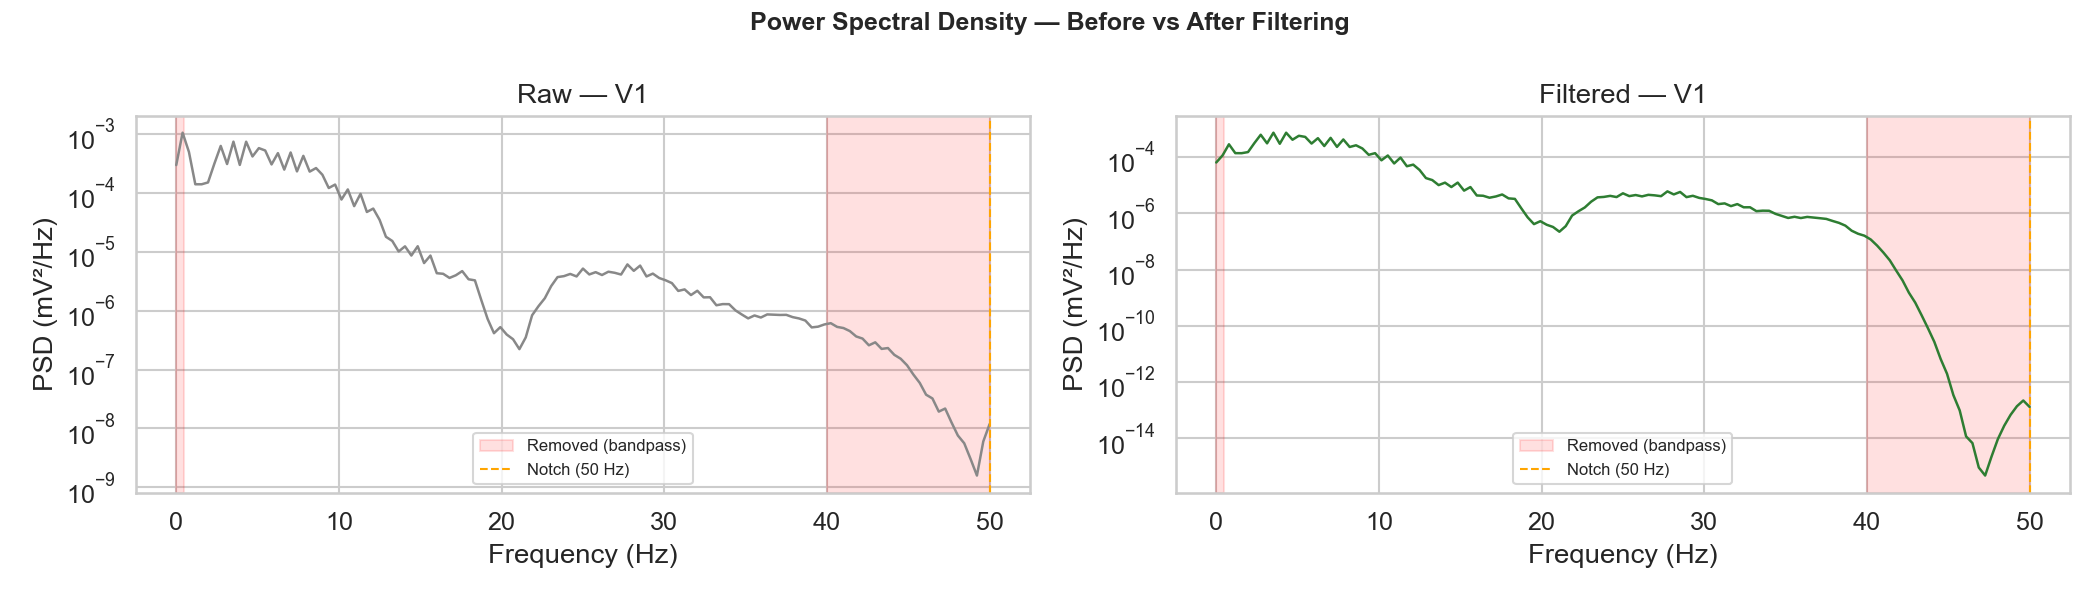
\includegraphics[width=\columnwidth]{preproc_psd_comparison.png}
  \caption{Power spectral density before (left) and after (right)
           filtering for Lead V1 of one Brugada patient.
           Out-of-band energy is effectively suppressed.}
  \label{fig:psd}
\end{figure}

% ══════════════════════════════════════════════════════════════════════════════
\begin{thebibliography}{99}

\bibitem{brugada1992right}
P.~Brugada and J.~Brugada,
``Right bundle branch block, persistent ST segment elevation and sudden
  cardiac death: a distinct clinical and electrocardiographic syndrome,''
\textit{Journal of the American College of Cardiology},
vol.~20, no.~6, pp.~1391--1396, 1992.

\bibitem{antzelevitch2005brugada}
C.~Antzelevitch \textit{et al.},
``Brugada syndrome: report of the second consensus conference,''
\textit{Heart Rhythm}, vol.~2, no.~4, pp.~429--440, 2005.

\bibitem{priori2013hrs}
S.~G.~Priori \textit{et al.},
``HRS/EHRA/APHRS expert consensus statement on the diagnosis and management
  of patients with inherited primary arrhythmia syndromes,''
\textit{Heart Rhythm}, vol.~10, no.~12, pp.~1932--1963, 2013.

\bibitem{hannun2019cardiologist}
A.~Y.~Hannun \textit{et al.},
``Cardiologist-level arrhythmia detection and classification in ambulatory
  electrocardiograms using a deep neural network,''
\textit{Nature Medicine}, vol.~25, no.~1, pp.~65--69, 2019.

\bibitem{ribeiro2020automatic}
A.~H.~Ribeiro \textit{et al.},
``Automatic diagnosis of the 12-lead ECG using a deep neural network,''
\textit{Nature Communications}, vol.~11, no.~1, p.~1760, 2020.

\bibitem{dataset}
F.~Pham \textit{et al.},
``Brugada-HUCA: A 12-lead ECG dataset for Brugada syndrome detection,''
\textit{PhysioNet}, 2023.

\bibitem{physionet}
A.~L.~Goldberger \textit{et al.},
``PhysioBank, PhysioToolkit, and PhysioNet: Components of a new research
  resource for complex physiologic signals,''
\textit{Circulation}, vol.~101, no.~23, pp.~e215--e220, 2000.

\bibitem{he2016deep}
K.~He, X.~Zhang, S.~Ren, and J.~Sun,
``Deep residual learning for image recognition,''
in \textit{Proc.\ IEEE CVPR}, pp.~770--778, 2016.

\bibitem{lundberg2017unified}
S.~M.~Lundberg and S.-I.~Lee,
``A unified approach to interpreting model predictions,''
in \textit{Advances in Neural Information Processing Systems}, vol.~30, 2017.

\bibitem{selvaraju2017grad}
R.~R.~Selvaraju \textit{et al.},
``Grad-CAM: Visual explanations from deep networks via gradient-based
  localization,''
in \textit{Proc.\ IEEE ICCV}, pp.~618--626, 2017.

\bibitem{wagner2020ptb}
P.~Wagner \textit{et al.},
``PTB-XL, a large publicly available electrocardiography dataset,''
\textit{Scientific Data}, vol.~7, no.~1, p.~154, 2020.

\bibitem{gal2016dropout}
Y.~Gal and Z.~Ghahramani,
``Dropout as a Bayesian approximation: Representing model uncertainty
  in deep learning,''
in \textit{Proc.\ ICML}, pp.~1050--1059, 2016.

\end{thebibliography}

\balance
\end{document}
